\Chapter{Új adatok előállítása, generatív modellek}
A generatív modellek alatt olyan gépi-tanulásos architektúrákat értünk, amelyek célja, hogy új adatokat állítsanak elő. A létrejött adatnak hasonlítania kell a tanítómintához, vagyis a generált minták eloszlásának közelítenie kell a valós adatok eloszlását. Az ilyen modelleknek meg kell tanulnia a tanítóminta jellegzetességeit és azt is, hogy ezen jellegeket a belső reprezentációjából hogyan tudná értelmezhető formában előállítani. A generatív modellek esetében ha a modell a tanítóminta képeit generálná csupán vissza pixel-pontosan, úgy a modell elveszti célját és egyfajta túltanulásnak (\textit{ovefitting}-nek) tekinthetnénk a jelenséget.

Az Autoencoder egy olyan statisztikai elveken alapuló architektúra, amelynek célja, hogy a tanítóhalmaz jellegzetességeit feltérképezze, és olyan formába kódolja a tulajdonságokat, hogy azokból az eredeti adat visszaállítható legyen. Az architektúra lényegében egy nehezen kezelhető sűrűségfüggvényt definiál, egy látens taggal, így ebben az esetben nem lehet közvetlenül optimalizálni, nem úgy mint például a pixelRNN/pixelCNN generatív modellek esetében \cite{oord2016conditional}, ahol az úgynevezett \textit{Evidence Lower Bound} (ELBO) mértékegységre kell optimalizálni\cite{oord2017neural}. Az architektúra két komponense az Encoder, amely előállítja a jellegvektorokat a bemenet alapján és a Decoder, amely a jellegvektorokból visszaállítja az adatot. Tehát ebben az esetben a cél az, hogy egy olyan reprezentációt készítsünk a tanítómintáról, amely alapján az teljes mértékben visszaállítható. Egyfajta tömörítési folyamatnak is felfogható az encoder működése. Egy módosított változattal az encoder által létrehozandó látens tér olyan formában áll elő, amelyből véletlenszerűen is vehetünk mintákat és dekódolva teljesen új adat áll elő. Ezt a módszert \textit{Vector Quantised-Variational AutoEncoder}-nek nevezték el, amely alkalmazható generatív modellként \cite{oord2017neural}.
Ha az autoencoder-t képek generálására kívánjuk felhasználni, úgy a helyreállított képeken egyfajta homályosságot figyelhetünk meg, amely a dekódolás során jelentkező információvesztésből adódik.

A \textit{Generative Adverserial Network} (GAN) \cite{goodfellow2014generative}, egy olyan generatív modell, amely nem a megszokott statisztikai alapokon optimalizál (mint például az Autoencoder vagy pixelRNN modellek), hanem játékelméleti megközelítést alkalmaz, így a modell tanítása is merőben másképp zajlik.
A tanulás során két neurális hálózat versenyzik egymással: egy generátor, amelynek az a szerepe, hogy a tanítómintákhoz hasonló adatot generáljon a bemeneti zajból és egy diszkriminátor, amely egy bináris osztályozó, amely a generátor által generált adatot vizsgálja és eldönti, hogy az valódi vagy hamis.
A tanítás során ezen két háló versenyzik egymással, együtt fejlődve. Az autoencoderhez képest a GAN-al generált képeken már nem figyelhető meg a homályosság, élesebb és fotórealisztikusabb képek generálására képes az eredmények alapján.

A generátor bemenete egy zajvektor, amelyet általában Gauss- vagy egyenletes eloszlásból állítunk elő. A zajnak a terét az irodalom látens térnek is nevezi, hiszen a tanítás során a modell megtanulja, hogy ezen többdimenziós tér egyes pontjaira milyen kimenetet generáljon. Vagyis ezzel lényegében kitölti a rendelkezésre álló tér tartományait a megtanult jellegzetességekkel. A betanított generátorral, optimális esetben, ezen tér bármely pontját mintavételezve a tanítóhalmazhoz hasonló adatokat generálhatunk. A hálózatok kialakításáról \aref{fig:aevsgan}. ábra ad áttekintést.

\begin{figure}[h]
\centering
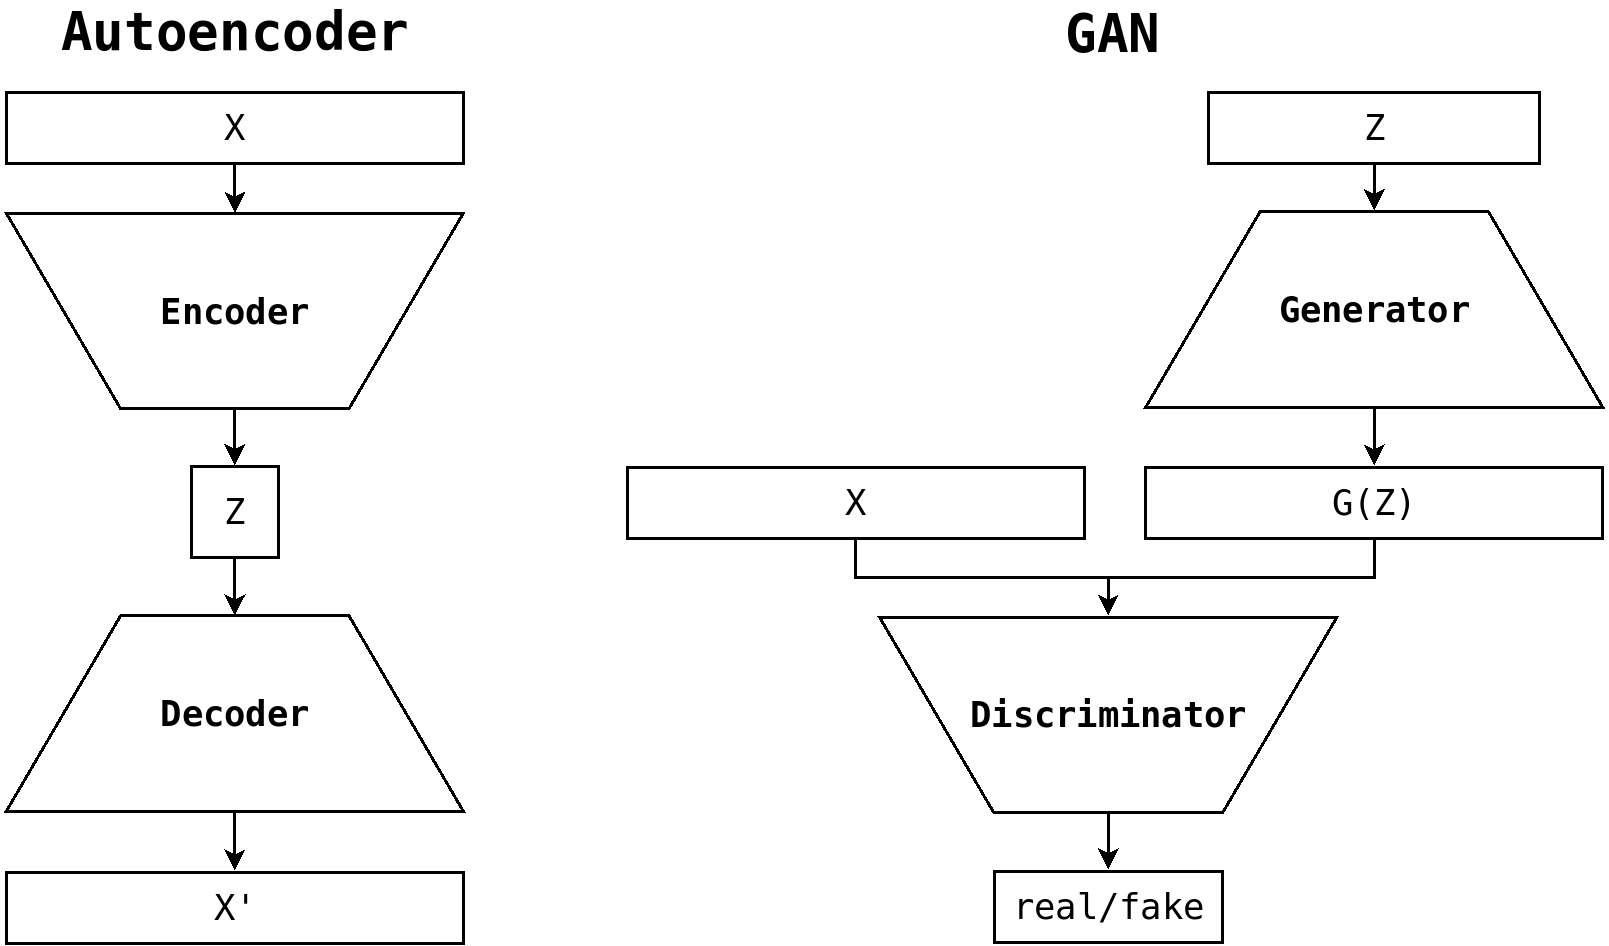
\includegraphics[width=12cm]{images/AEvsGAN.png}
\caption{Az Autoencoder és a GAN}
\label{fig:aevsgan}
\end{figure}

\Section{GAN modell tanítása}

A továbbiakban a következő jelöléseket használom: legyen $D$ a diszkriminátor, $G$ pedig a generátor.
Ha a legegyszerűbb esetet vizsgáljuk és csak a képek rendezetlen halmazára tanítjuk a modellt, mindenféle kiegészítő információ és annotáció nélkül, akkor a tanítás a következő pontokban leírtaknak megfelelően zajlik.

\SubSection{Hibafüggvények}

A $G$ és $D$ hibájának számolása a bináris kereszt-entrópián alapszik.
A bináris kereszt-entrópia hibafüggvény a következőképpen írható fel:
$$L(\hat y, y) = y \cdot \log \hat y + (1-y) \cdot \log (1 - \hat y),$$
ahol $\hat y$ a predikció, $y$ pedig a valós címke.

A Kerasban található implementáció egy segédfüggvényt ad vissza, amelyet különféle paraméterekkel inicializálhatunk.
\begin{python}
cross_entropy = keras.losses.BinaryCrossentropy(from_logits=True)
\end{python}
A \texttt{from\_logits=True} paraméter esetén a keresztentrópia számolásnál nem szükséges a diszkriminátor modellnek tartalmaznia az utolsó sigmoid aktivációs függvényét, ami így egy úgynevezett \textit{Logits} kimenettel fog rendelkezni. A számolás során a kimeneti értékekre alkalmazódik ebben az esetben a szigmoid függvény egy fajtája.

\SubSection{Diszkriminátor hibafüggvénye}

A $G$ generátor egy $z \in \mathbb{R}^n, n \geq 1$ bemeneti zajvektor alapján előállít egy generált adatot $G(z)$.
A $D$ diszkriminátor egy bináris osztályozó, amelynek feladata, hogy az $x$ és $G(z)$ bemeneteit osztályozza.
$D(x)$ esetén 1, $D(G(z))$ esetén pedig 0 címkét várunk.
A hibafüggvény számolása két lépésben történik a kétféle bemenet miatt.

$D(x)$-re nézve a kereszt-entrópia a következő:
$$L(D(x), 1) = 1 \cdot \ln D(x) + (1 - 1) \cdot \ln(1 - D(x)) = \ln D(x),$$
vagyis jelen esetben $D$-nek a $\ln(D(x))$-et kell maximalizálnia.

$D(G(z))$-re nézve a kereszt-entrópia a következő:
$$L(D(G(z)), 0) = 0 \cdot \ln D(G(z)) + (1 - 0) \cdot \ln(1 - D(G(z))) = \ln(1- D(G(z))),$$
vagyis a $\ln(1 - D(G(z)))$-t kell maximalizálnia.

Egyetlen mintára a hibafüggvény a következőképpen néz ki:
$$\max V(D) = \ln D(x) + \ln(1 - D(G(z)),$$
Batch-ra nézve:
$$\max V(D) = \mathbb{E}_{x \sim P(x)} \left[\ln D(x) \right] + \mathbb{E}_{z \sim P(z)} \left[\ln(1 - D(G(z))) \right],$$
ahol a $P(x)$ a valószínűségi eloszlása a tanítóhalmaznak, $P(z)$ a valószínűségi eloszlása a $z$ zajvektornak (látens térnek).

A hibafüggvény implementációja összességében az alábbi:
\begin{python}
def discriminator_loss(real_output, fake_output):
    real_loss = cross_entropy(tf.ones_like(real_output), real_output)
    fake_loss = cross_entropy(tf.zeros_like(fake_output), fake_output)
    
    total_loss = real_loss + fake_loss
    return total_loss
\end{python}

\SubSection{Generátor hibafüggvénye}

A $G$ generátor feladata az, hogy megtévessze a $D$ diszkriminátort azáltal, hogy a tanítóhalmazhoz hasonló adatokat generáljon.
Vagyis a $G$ érdeke az, hogy a $D(G(z))$ 1-es címkét kapjon 0 helyett.

A bináris keresztentrópia egy mintára:
$$L(D(G(z)), 0) = \ln(1 - D(G(z)).$$
$D$ minimalizálni kívánja a $D(G(z))$-t, míg a $G$ maximalizálni szándékozik azt.

A $G$ a tanítás során sosem fog valódi adatot látni, csupán a diszkriminátor hibáiból fog tanulni.

A generátorhoz tartozó hibafüggvény implementációja:
\begin{python}
def generator_loss(fake_output):
    return cross_entropy(tf.ones_like(fake_output), fake_output)
\end{python}

A GAN hálózat tanítása során $D$ és $G$ egy minimax játékot játszanak a $V(G, D)$ értékfüggvénnyel. Ez formálisan:
$$\min_{G}\max_{D}V(D, G) =  \mathbb{E}_{x \sim P(x)} \left[\ln D(x) \right] + \mathbb{E}_{z \sim P(z)} \left[\ln(1 - D(G(z))) \right].$$

\SubSection{Optimalizáló módszer}
A GAN modell súlyait a sztochasztikus gradiens algoritmussal szokás frissíteni.

A Generátort és a Diszkriminátort a hibafüggvények alapján kiszámolt gradiensek alapján külön-külön kell tanítani. Különféle szerzők különböző optimalizáló módszerek használatát javasolják, az Adam és az RMSProp a két legnépszerűbb módszer \cite{kingma2014adam}.

A saját implementációimban az Adam optimalizáló módszert alkalmaztam. A módszer legfontosabb paramétere a \textit{learning-rate}, vagyis a tanulási mérték. A 0.0001 learning-rate érték megfelelőnek tűnt a modelljeim tanítása során.

Az alábbi kódrészlet segítségével inicializálhatunk egy-egy példányt az Adam optimalizálóból a generátornak és a diszkriminátornak.

\begin{python}
generator_optimizer = keras.optimizers.Adam(1e-4)
discriminator_optimizer = keras.optimizers.Adam(1e-4)
\end{python}


\SubSection{Tanítási lépés}
A GAN esetében a hálózat paraméterei közé tartozik a mini-batch elemszáma is. Mini-batch alatt a tanítóhalmaz egy bizonyos elemszámú mintát tartalmazó szeletét értjük. A mini-batch-ek alkalmazása azért lényeges, hogy egy tanítási lépés során a modell ne lássa a teljes tanítóhalmazt. A hálózat tanításához általában sok mintára van szükségünk, így az egy darabban való tanítás igen nehézkes és számításigényes lenne. De nem csupán ez jelenti a fő veszélyt, Ha egy lépésben láthatná a diszkriminátor az összes képet, akkor túlságosan is megnőne a teljesítménye és a generátornak esélye sem lenne felzárkózni. A mini-batch-eken való tanítás tehát elengedhetetlen része a tanítási folyamatnak és a megfelelő ütemű tanulás biztosításának.
A fellelhető irodalomban a mini-batch-et néhány esetben röviden batch-nek nevezik. Viszont a batch egyes irodalmakban a teljes dataset-et jelöli, így az egyértelműség kedvéért minden esetben kiírom, hogy mini-batch.

%% GAN 2014 cikkből

Legyen $m$ a mini-batch elemszáma $m \in \mathbb{N}$
A GAN hálózat egy tanítási lépése a következő műveletekből áll \cite{goodfellow2014generative}:
\begin{enumerate}
\item Hozzunk létre $m$ darab zajmintát $(z_1, \ldots, z_m)$ normális eloszlásból $P_g(z)$.
\item A tanítóhalmazból emeljük ki a soron következő $m$ darab tanítómintát (képet), és ezt jelöljük $(x_1, \ldots, x_m)$-el. % $P_{\text{data}}(x)$
\item Frissítsük a $D$ diszkriminátort a sztochasztikus gradiens emelkedésével, amelynek értéke
$$ \nabla \theta_d \frac{1}{m} \sum_{i=1}^{m} \left[\log D(x_i) + \log(1 - D(G(z_i))) \right].$$
\item  Frissítsük a $G$ generátort a sztochasztikus gradiens süllyesztéssel:
$$ \nabla \theta_d \frac{1}{m} \sum_{i=1}^{m} \log(1 - D(G(z_i))).$$
\end{enumerate}

A GAN részeit tehát külön-külön tanítjuk, hiszen különböző neurális hálókról van szó. Az eredeti cikkben is javaslatot tesznek arra, hogy a $D$-t esetleg több lépésben is lehetne tanítani, majd a $G$-t egyetlen lépésben frissíteni.
Különböző tanítási stratégiákban ez is egy szabad paraméter lehet. Számomra megfelelő volt az 1:1-es tanítási lépés alkalmazása is. Viszont több cikkben is vizsgálják ezt, mint lehetséges beállítást.
A tanítás hossza természetesen függ az adathalmaztól és annak méretétől, az alkalmazott mini-batch mérettől, a modellben található paraméterektől és az optimalizáló eljárástól.

A TensorFlow-ban és Keras-ban történő tanítási lépés megvalósítása a következő kódrészletben figyelhető meg. A \texttt{@tf.function} annotáció segítségével jelezhetjük a TensorFlow backend-nek, hogy az annotációval ellátott függvényt fordítsa le. Az annotáció használata a kritikus, nagy erőforrás-igényű és ismétlődő számolásoknál a futásidőt csökkentheti. Az függvény első meghívásánál felállítja a függőségi vagy hívási gráfot is, ezzel is csökkentve a futásidőt.

\begin{python}
@tf.function
def train_step(images):
    noise = random.normal([batch_size, latent_dim])
    with GradientTape() as gen_tape, GradientTape() as disc_tape:
        generated_images = generator(noise, training=True)
        real_output = discriminator(images, training=True)
        fake_output = discriminator(generated_images, training=True)
        gen_loss = generator_loss(fake_output)
        disc_loss = discriminator_loss(real_output, fake_output)
    gradients_of_generator = gen_tape.gradient(
        gen_loss, generator.trainable_variables
    )
    gradients_of_discriminator = disc_tape.gradient(
        disc_loss, discriminator.trainable_variables
    )
    generator_optimizer.apply_gradients(
        zip(gradients_of_generator,
        generator.trainable_variables)
    )
    discriminator_optimizer.apply_gradients(
        zip(gradients_of_discriminator,
        discriminator.trainable_variables)
    )
\end{python}

A tanítás ciklus függvénye az alábbi módon nézhet ki. Ehhez olyan dataset-re lesz szükségünk, amely mini-batch-eket tartalmaz.

A tanítás Python függvény formájában a következőképpen foglalható össze:
\begin{python}
def train(dataset, epochs):
    for epoch in range(epochs):
        for (batch, image_batch) in enumerate(dataset):
            train_step(image_batch)
\end{python}

\Section{Képeket előállító GAN modell}

Ezen architektúra természetesen a mai eredmények mellett egyszerűnek tűnhet elsőre, viszont a későbbi, fejlettebb architektúrákban többségében megfigyelhető, hogy ezen modellt vették alapul. Természetesen az architektúra egy igen egyszerű kiegészítést kínált az eredeti GAN hálózatra: konvolúciós rétegeket alkalmaz a rejtett rétegekben mind a Generátor, mind a Diszkriminátor esetében. A konvolúciós rétegek segítségével a képeken lévő összefüggő pixelek kapcsolatairól pontosabb reprezentációt kaphatunk, így képek generálásához is hasznos lehet a módszer.

\begin{figure}[h]
\centering
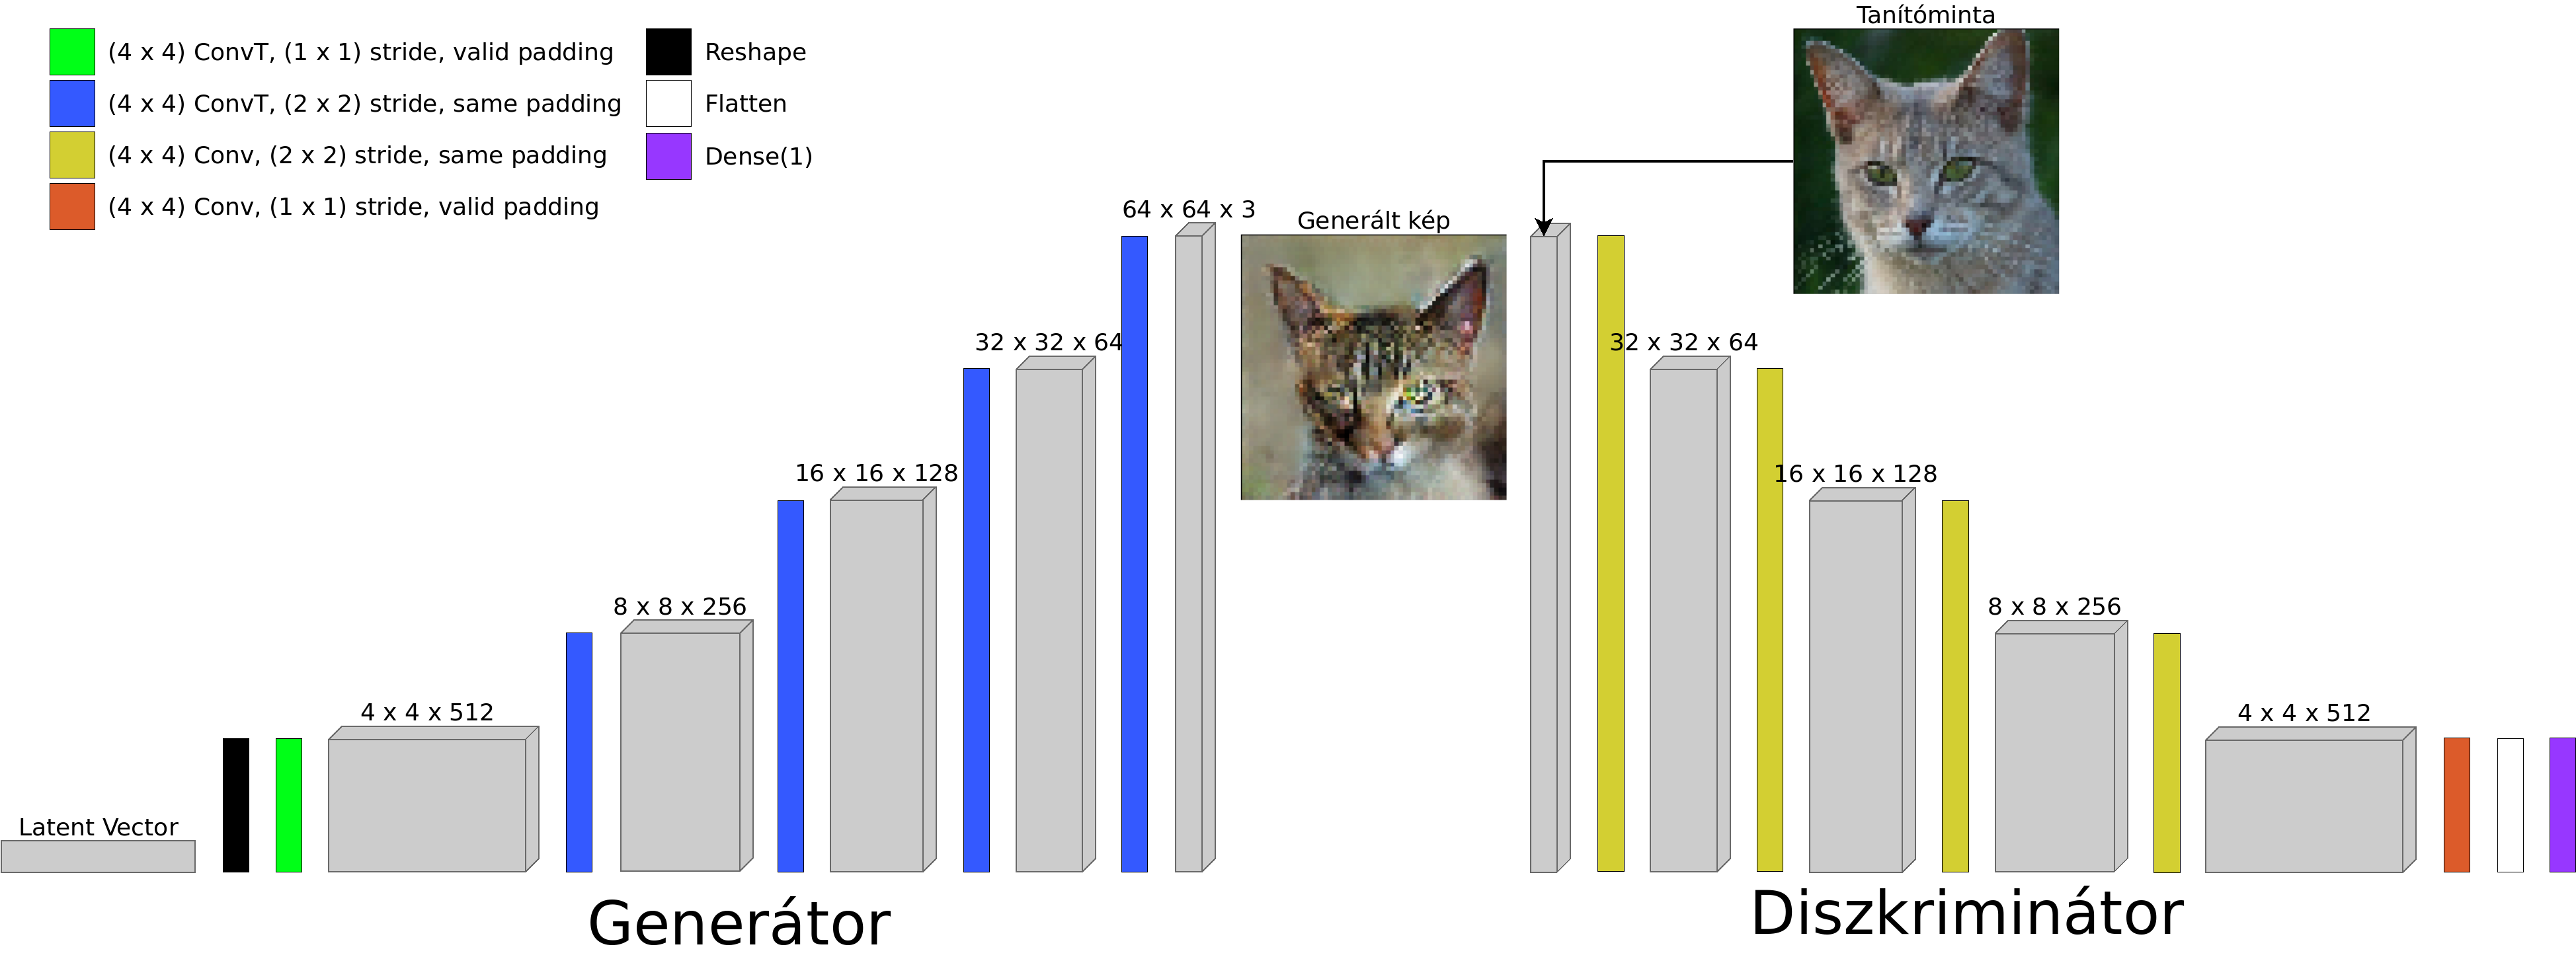
\includegraphics[width=15cm]{images/DCGAN.png}
\caption{DCGAN architektúra}
\label{fig:dcgan}
\end{figure}

\SubSection{Generátor}

Az osztályozáshoz használt konvolúciós hálókkal ellentétben a Generátorban a kisebb felbontás felől haladunk a nagyobb felbontásig.
A generátor modellem első implementációjában \textit{Dekonvolúciós} rétegeket alkalmaztam, amelyet \textit{Transzponált konvolúciós} rétegnek is nevezhetünk. A dekonvolúció a konvolúció ellentettje, vagyis a feladata, hogy egy alacsonyabb dimenziójú reprezentációt magasabb dimenzióba emeljen. Segítségével minden rejtett réteg kimenete egy nagyobb felbontású kép lesz. Tehát a hálónak jelen esetben meg kell tanulnia a rétegekben az optimális felbontás-növelést. Előre megadott paraméterek a filterek darabszáma, a kernel mérete, a strides és a padding. Ha a padding-et "same"-re és ha a strides paramétert $2 \times 2$-esnek választjuk, úgy a réteg kimenetén megjelenő kép felbontása dimenziónként kétszerese lesz a bemeneti oldalon megfigyelhető képnek. A rejtett rétegekben ReLU aktivációs függvényt (\ref{fig:relu}. ábra) használtam, a neuronok kezdő értékeit a He inicializációs technikával \cite{he2015delving} állítottam be.

\begin{figure}[h]
\centering
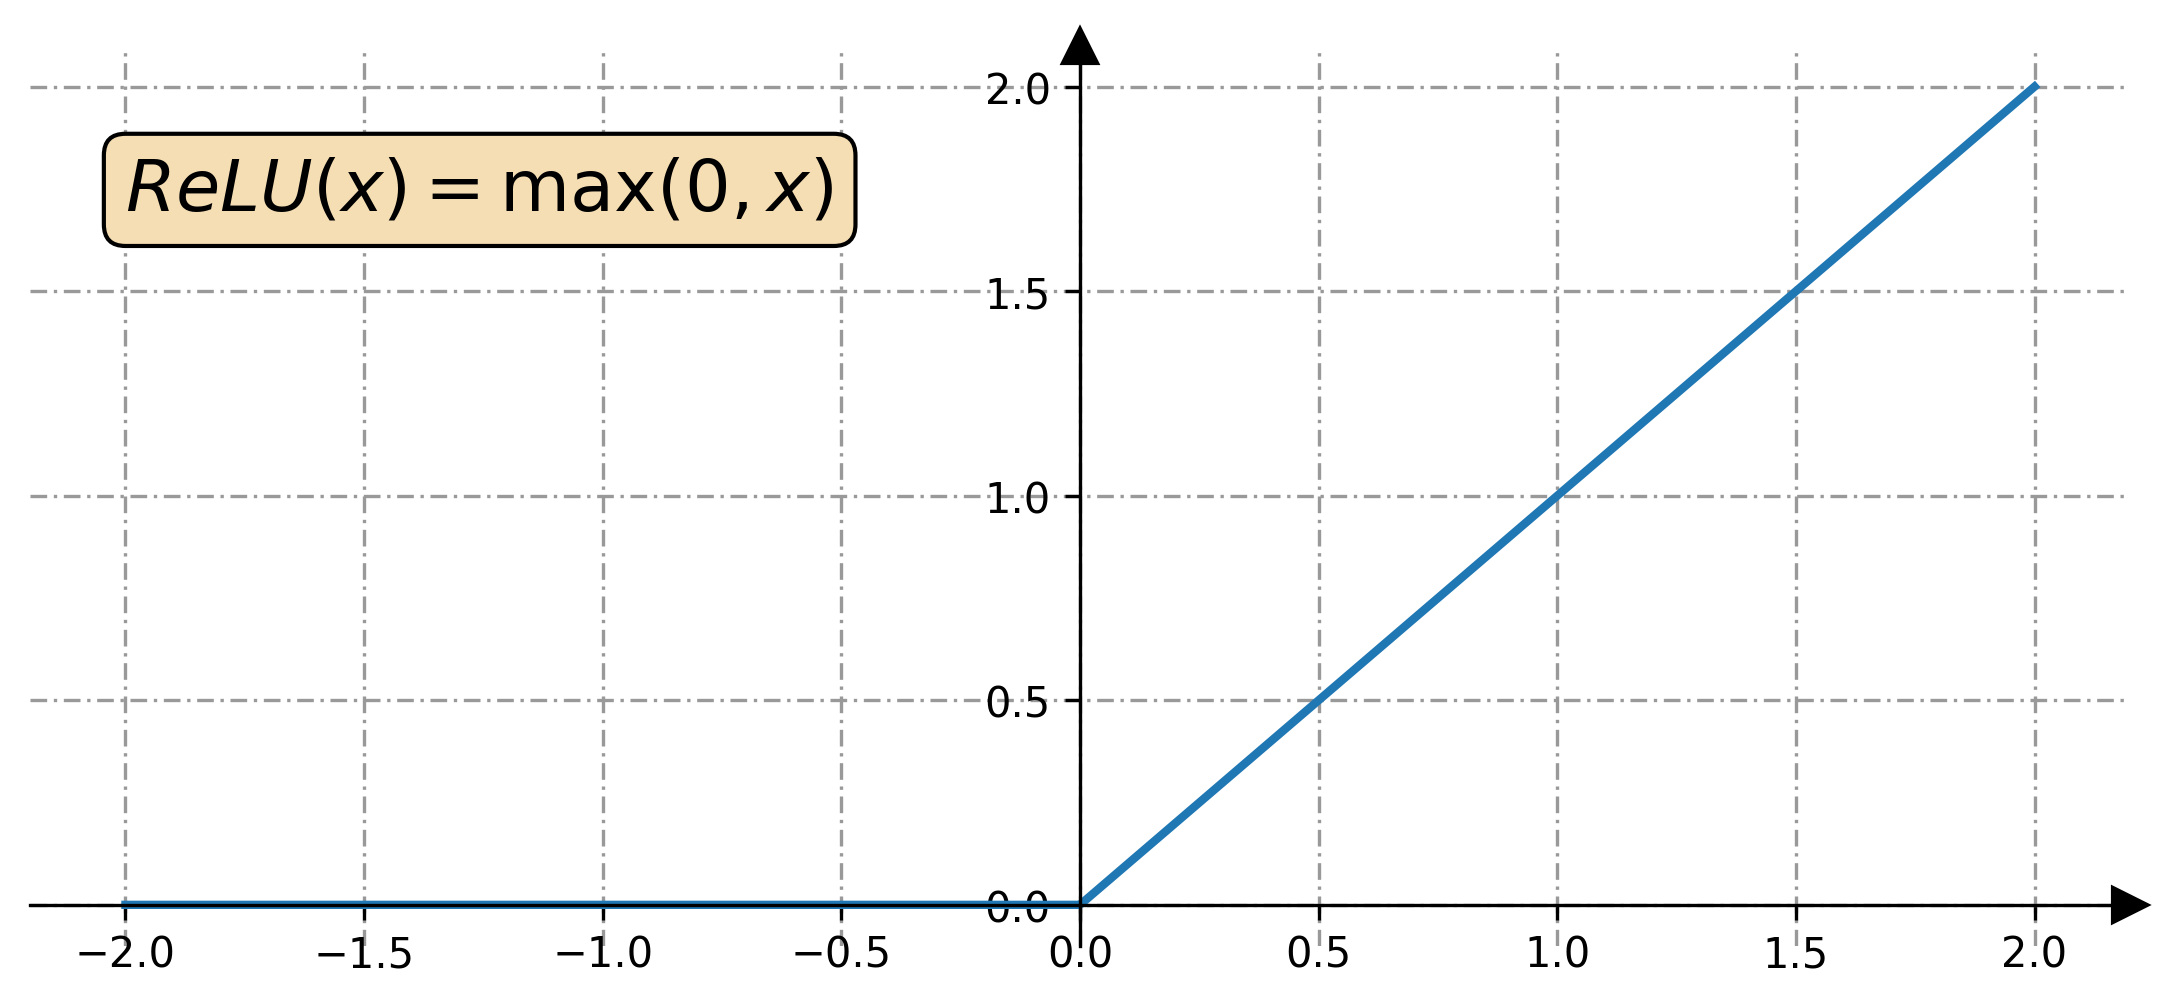
\includegraphics[width=10cm]{images/relu.png}
\caption{ReLU aktivációs függvény}
\label{fig:relu}
\end{figure}

A tanításhoz célszerű a kép pixeleinek intenzitását normalizálni a $[-1, 1]$ intervallumra lebegőpontos értékekre. A Generátor is ebben az intervallumban fogja a képek pixeleit generálni a hiperbolikus tangens kimeneti aktivációs függvényéből adódóan. A megjelenítéshez később természetesen denormalizálnunk kell a generált képek pixelértékeit a $[0, 255]$ tartományra.

A Generátor modell bemenetként az előre definiált látens tér dimenziójával megegyező dimenziójú zajt kap, vagyis annak a $z_n$ dimenziószámú térnek egy pontját. Majd ezen bemeneti zaj segítségével állítja össze a megfelelő kimeneti képet. A tanulás során tehát a látens tér tartományaihoz rendeli a tanult jellegzetességeket és a látens teret mintavételezve dekódolható a Generátor segítségével a ponthoz tartozó kép.

A bemeneti zaj egy \textit{Reshape} rétegen megy keresztül, amelyben a látens tér dimenziószámát átformázza egy $1 \times 1 \times z_n$ dimenziójú mátrixszá. Ezen réteg kimenetével a későbbi dekonvolúciós rétegek már tudnak dolgozni.
Ezután az első dekonvolúciós rétegen megy át a kapott mátrix, amely 512 darab filtert tartalmaz, $4 \times 4$-es kernelméretekkel dolgozik és 'valid' paddingot használ. Az aktivációs függvénye ReLU a már említett He inicializálással. Ezen lépés arra szolgál, hogy a látens térből előállítson egy $4 \times 4 \times 512$ alakú tensor-t, amely az első, legkisebb felbontású képünknek tekinthetjük ebben az esetben, ahol a színcsatornák száma 512 és a felbontása pedig $4 \times 4$.

A Generátorban ezután $2 \times 2$-es stride értékeket használva same padding-gel a kívánt felbontásig dekonvolúciós rétegeken keresztül növekszik a felbontás. A kernelméretét a rétegekben egységesen $4 \times 4$-ra állítottam be. Az aktivációs függvény szintén ReLU. A rétegekben haladva a filterek darabszáma pedig feleződik. A filterek optimális számára csupán csak empirikus eredményeket találtam a szakirodalomban. A felezéses eljárással a paraméterek száma viszonylag alacsonyabban tartható és a tanítás ideje is lecsökken.

A kimeneti képnek olyan tulajdonságokkal kell rendelkeznie, mint a tanítómintában szeplő képeknek. Például ha a tanítóminta színes képekből áll, \textit{RGB} színkeveréssel, vagyis három színcsatornával, úgy a Generátor kimenetén is ilyen képekre van szükségünk. Mivel az említett dekonvolúciós rétegek több mint 3 színcsatornával dolgoztak, a megjeleníthetőség miatt szükséges tehát az utolsó dekonvolúciós rétegben a 3 darab filter, amely egyaránt transzponálja az előző réteg reprezentációit az egyel magasabb felbontás értékbe, és a csatornák számát pedig 3-ra állítja.
Egyes GAN architektúrákban ez az utolsó réteg csupán a 3 színcsatornába vetítést végzi el konvolúciós réteggel és szokás \textit{toRGB} rétegnek is nevezni \cite{karras2017progressive, karras2019style, karnewar2020msg}. Viszont jelen esetben egyúttal a felbontást is növeli a példámban szereplő utolsó réteg, ha $1 \times 1$-es stride értékkel rendelkezne ez a dekonvolúciós réteg, akkor valójában úgy működne, mint egy konvolúciós réteg, és tényleg csak a csatornák számát változtatná meg. Viszont akkor szükség lenne még egy felbontásnövelő rétegre, amely tovább növelné a paraméterek számát.

Végül a hiperbolikus tangens aktivációs függvény (\ref{fig:tanh}. ábra) az eredményeket a $[-1, 1]$ intervallumba transzformálja.

\begin{figure}[h]
	\centering
	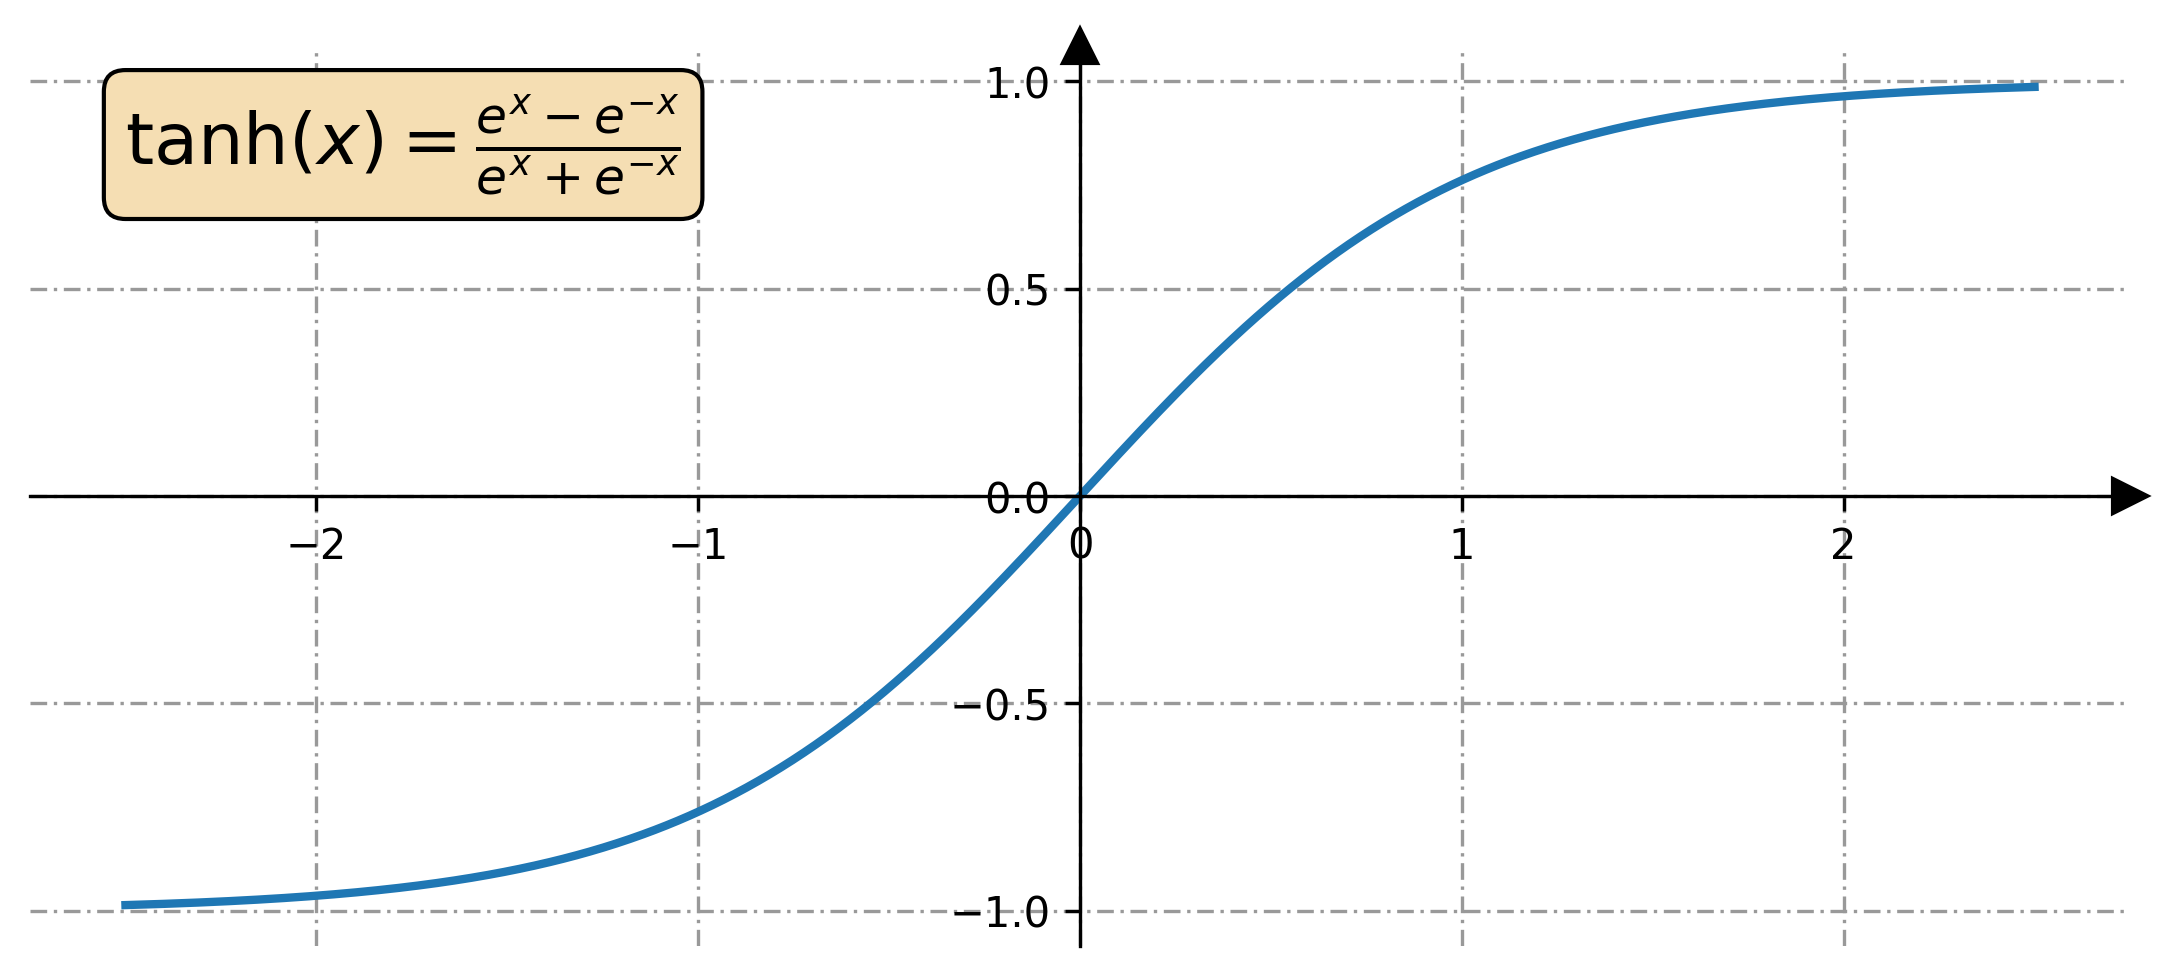
\includegraphics[width=10cm]{images/tanh.png}
	\caption{Hiperbolikus tangens aktivációs függvény}
	\label{fig:tanh}
\end{figure}

Az alábbi kódrészletben látható a felvázolt generátor architektúra megvalósítása a Keras \textit{Sequential API}-ja segítségével.

\begin{python}
generator = keras.Sequential([
    keras.layers.Reshape((1, 1, 100), input_shape=[100]),
    keras.layers.Conv2DTranspose(512, (4, 4), (1, 1), "valid",
                                 activation="relu",
                                 kernel_initializer="he_normal"),
    keras.layers.Conv2DTranspose(256, (4, 4), (2, 2), "same",
                                 activation="relu",
                                 kernel_initializer="he_normal"),
    keras.layers.Conv2DTranspose(128, (4, 4), (2, 2), "same",
                                 activation="relu",
                                 kernel_initializer="he_normal"),
    keras.layers.Conv2DTranspose(64, (4, 4), (2, 2), "same",
                                 activation="relu",
                                 kernel_initializer="he_normal"),
    keras.layers.Conv2DTranspose(3, (4, 4), (2, 2), "same",
                                 activation="relu"),
    keras.layers.Activation("tanh")
])
\end{python}


\SubSection{Diszkriminátor}

A Diszkriminátor modell lényegében egy bináris osztályozó, amely eldönti, hogy a bemenetül kapott kép valódi-e vagy hamis. A bemeneti kép konvolúciós rétegeken megy végig, kinyerve a jellegzetességeket és felállítva egy olyan belső reprezentációt, amely alapján az utolsó \textit{dense} réteg megfelelő kimenettel tud rendelkezni. A képen található mintázatokat a konvolúciós rétegek filterek segítségével tanulják meg, amelyek megadott kernelméretekben pásztázzák végig a bemenetet. Így az egyes konvolúciós rétegek kimeneteként egy olyan reprezentáció jön létre a bemeneti képről, amelyben érvényesülnek a pixeleket körülölelő további pixelek kapcsolatai is. Ezáltal az utolsó előtti réteg, a szerializáció (\textit{Flattening}) kevésbé fogja a kép tartalmára vonatkozó információt rontani. Mivel a tanítóminta képeinek pixelértékeit normalizáltuk a $[-1, 1]$ intervallumra, így a diszkriminátor a bemenetén is ilyen tulajdonságú képeket vár. A Diszkriminátor felépítésben hasonlít a Generátorhoz, lényegében annak tükörképeként képzelhetjük el. Viszont a dekonvolúciós rétegek helyett konvolúciós rétegeket alkalmazunk benne a jellegzetességek kinyerésére. Majd ha eljutunk a kívánt dimenziószámig, egy teljesen összekötött rétegben hozza meg a modell a döntést.

A generátorhoz hasonlóan az alábbi kódrészlet bemutatja a felvázolt diszkriminátor Keras Sequential API-val történő megvalósítását:

\begin{python}
discriminator = keras.Sequential([
    keras.layers.Conv2D(64, (4, 4), (2, 2), "same",
                        input_shape=(64, 64, 3), activation="relu",
                        kernel_initializer="he_normal"),
    keras.layers.Conv2D(128, (4, 4), (2, 2), "same", activation="relu",
                        kernel_initializer="he_normal"),
    keras.layers.Conv2D(256, (4, 4), (2, 2), "same", activation="relu",
                        kernel_initializer="he_normal"),
    keras.layers.Conv2D(512, (4, 4), (2, 2), "same", activation="relu",
                        kernel_initializer="he_normal"),
    keras.layers.Conv2D(100, (4, 4), (1, 1), "valid", activation="relu"),
    keras.layers.Flatten(),
    keras.layers.Dense(1)
])
\end{python}

Mint a kódrészletből is látható, az utolsó teljesen összekötött rétegnek nincsen aktivációs függvénye, \textit{Logits} kimenettel rendelkezik. A szigmoid függvényt a keresztentrópia számolásnál alkalmazzuk majd a dense réteg kimenetére.

\Aref{tab:gen_disc_params}. táblázatokban összefoglaltam az architektúra felépítését.

\begin{table}[h!]
	\centering
\caption{A hálózatokhoz tartozó rétegek és paramétereik}
\label{tab:gen_disc_params}
\medskip
\begin{tabular}{c c}
\scriptsize{
\begin{tabular}{@{\extracolsep{5pt}} |l c r| }
	\hline
	\multicolumn{3}{|c|}{\textbf{Generátor}} \\
	\hline
	Réteg & Aktivációs fv & Kimenet\\
	\cline{1-1} \cline{2-2} \cline{3-3}
	Input & - & (100)\\
	Reshape & - & (1, 1, 100)\\
	(4x4) ConvT & ReLU & (4, 4, 512)\\
	(4x4) ConvT & ReLU & (8, 8, 256)\\
	(4x4) ConvT & ReLU & (16, 16, 128)\\
	(4x4) ConvT & ReLU & (32, 32, 64)\\
	(4x4) ConvT & tanh & (64, 64, 3)\\
	\hline
	\multicolumn{3}{|r|}{Paraméterek száma: \textbf{3.5 millió}} \\
	\hline
\end{tabular}}

&\scriptsize{
\begin{tabular}{@{\extracolsep{5pt}} |l c r| }
	\hline
	\multicolumn{3}{|c|}{\textbf{Diszkriminátor}} \\
	\hline
	Réteg & Aktivációs fv & Kimenet\\
	\cline{1-1} \cline{2-2} \cline{3-3}
	Input & - & (64, 64, 3)\\
	(4x4) Conv & ReLU & (32, 32, 64)\\
	(4x4) Conv & ReLU & (16, 16, 128)\\
	(4x4) Conv & ReLU & (8, 8, 256)\\
	(4x4) Conv & ReLU & (4, 4, 512)\\
	(4x4) Conv & ReLU & (1, 1, 100)\\
	Flatten & - & (100)\\
	Dense(1) & - & (1)\\
	\hline
	\multicolumn{3}{|r|}{Paraméterek száma: \textbf{3.5 millió}} \\
	\hline
\end{tabular}}

\end{tabular}
\end{table}

\SubSection{Tanítás, mérések}

A felvázolt architektúrát az AFHQ dataset-en, Adam optimalizációs módszerrel, 0.0004 \textit{learning rate} hiperparaméter mellett tanítva a hibaértékek \aref{fig:mini-batch_loss_plot}. ábrához hasonlóan alakulnak.

\begin{figure}[h]
\centering
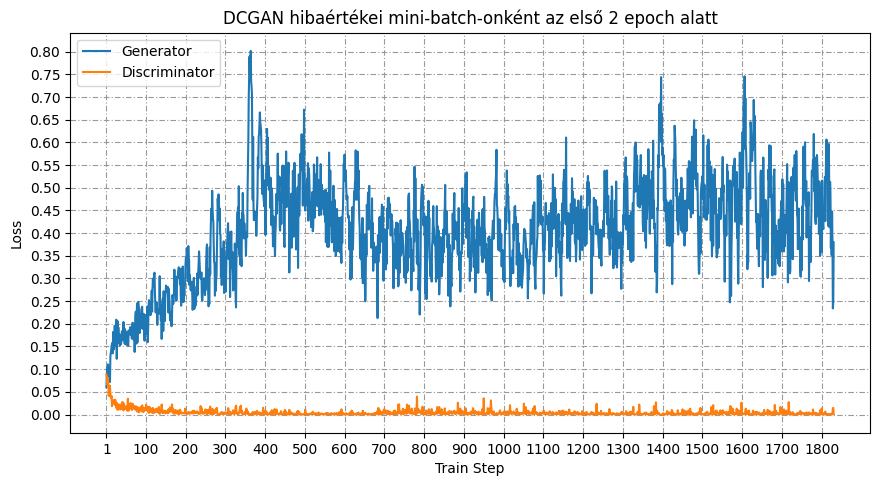
\includegraphics[width=15cm]{images/miniloss.png}
\caption{Hibaértékek mini-batch-enként}
\label{fig:mini-batch_loss_plot}
\end{figure}

Egy tanítási lépés egy mini-batch-en történő tanítást jelent, egy epoch pedig az összes mini-batch-en való tanítást jelenti.
Ha csak a nyers hibaértékre tekintünk, akkor azt figyelhetjük meg, hogy a tanítási lépések között erősen oszcillálnak az értékek. Kijelenthetjük a látott eredmények alapján, hogy a tanítás valóban nem stabil és látszólag tetszőlegesen módon változhatnak az értékek.
A szemléltetés kedvéért \aref{fig:epoch_loss_plot}. ábrán a mini-batch-eken számolt hibaértékek átlagait figyelhetjük meg epoch-onként.

\begin{figure}[h]
\centering
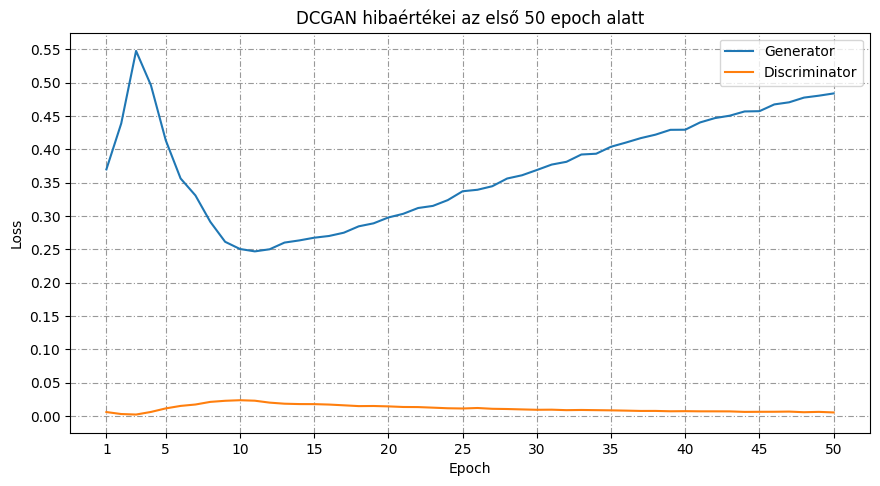
\includegraphics[width=15cm]{images/epochloss.png}
\caption{Hibaértékek epoch-onként}
\label{fig:epoch_loss_plot}
\end{figure}

Így simább görbéket kapunk, viszont erősen torzít az ábra, hiszen a GAN tanítási folyamata nem ilyen rendezett, mint ahogyan az első ábrán is láthattuk.
A hibaértékek változását vizsgálva megfigyelhető a versengés, vagyis hogy a két hálózat hibái mennyire ellentétesen mozognak az epoch-ok alatt. Mivel a tanulás során függőség van a két hálózat között, így ha a diszkriminátor egy vizsgált epoch alatt rosszabbul teljesítene a korábbi eredményekhez képest, akkor az a generátor javára válik és annak hibaértéke alacsonyabb lesz és fordítva. A generátor hibái többszörösek lehetnek a diszkriminátor hibáinak, de ez a jelenség teljesen természetes, hiszen a generátor lényegében a másik hálózat hibáiból tud csak tanulni, mivel a tanulás során nem látja a tanítóminta elemeit. A generátorban megfigyelhető, egyre növekvő hibaérték ellenére a generált képek minősége és részletezettsége is növekedni fog.

A hibaértékekből nem vonhatunk le pontos következtetéseket, így a fenti ábrák csupán szemléltetésképp készültek el. A GAN teljesítményének mérésére egyéb ajánlások jelentek meg, ilyen az \textit{Inception Score} \cite{salimans2016improved} és az \textit{Fréchet Inception Distance} \cite{heusel2017gans}.

\SubSection{Az architektúra gyengeségei, problémái}

A felvázolt architektúra tanítása során különféle problémák jelentkezhetnek, amelyek a végeredményt kisebb nagyobb mértékben ronthatják.

\begin{figure}[h]
	\centering
	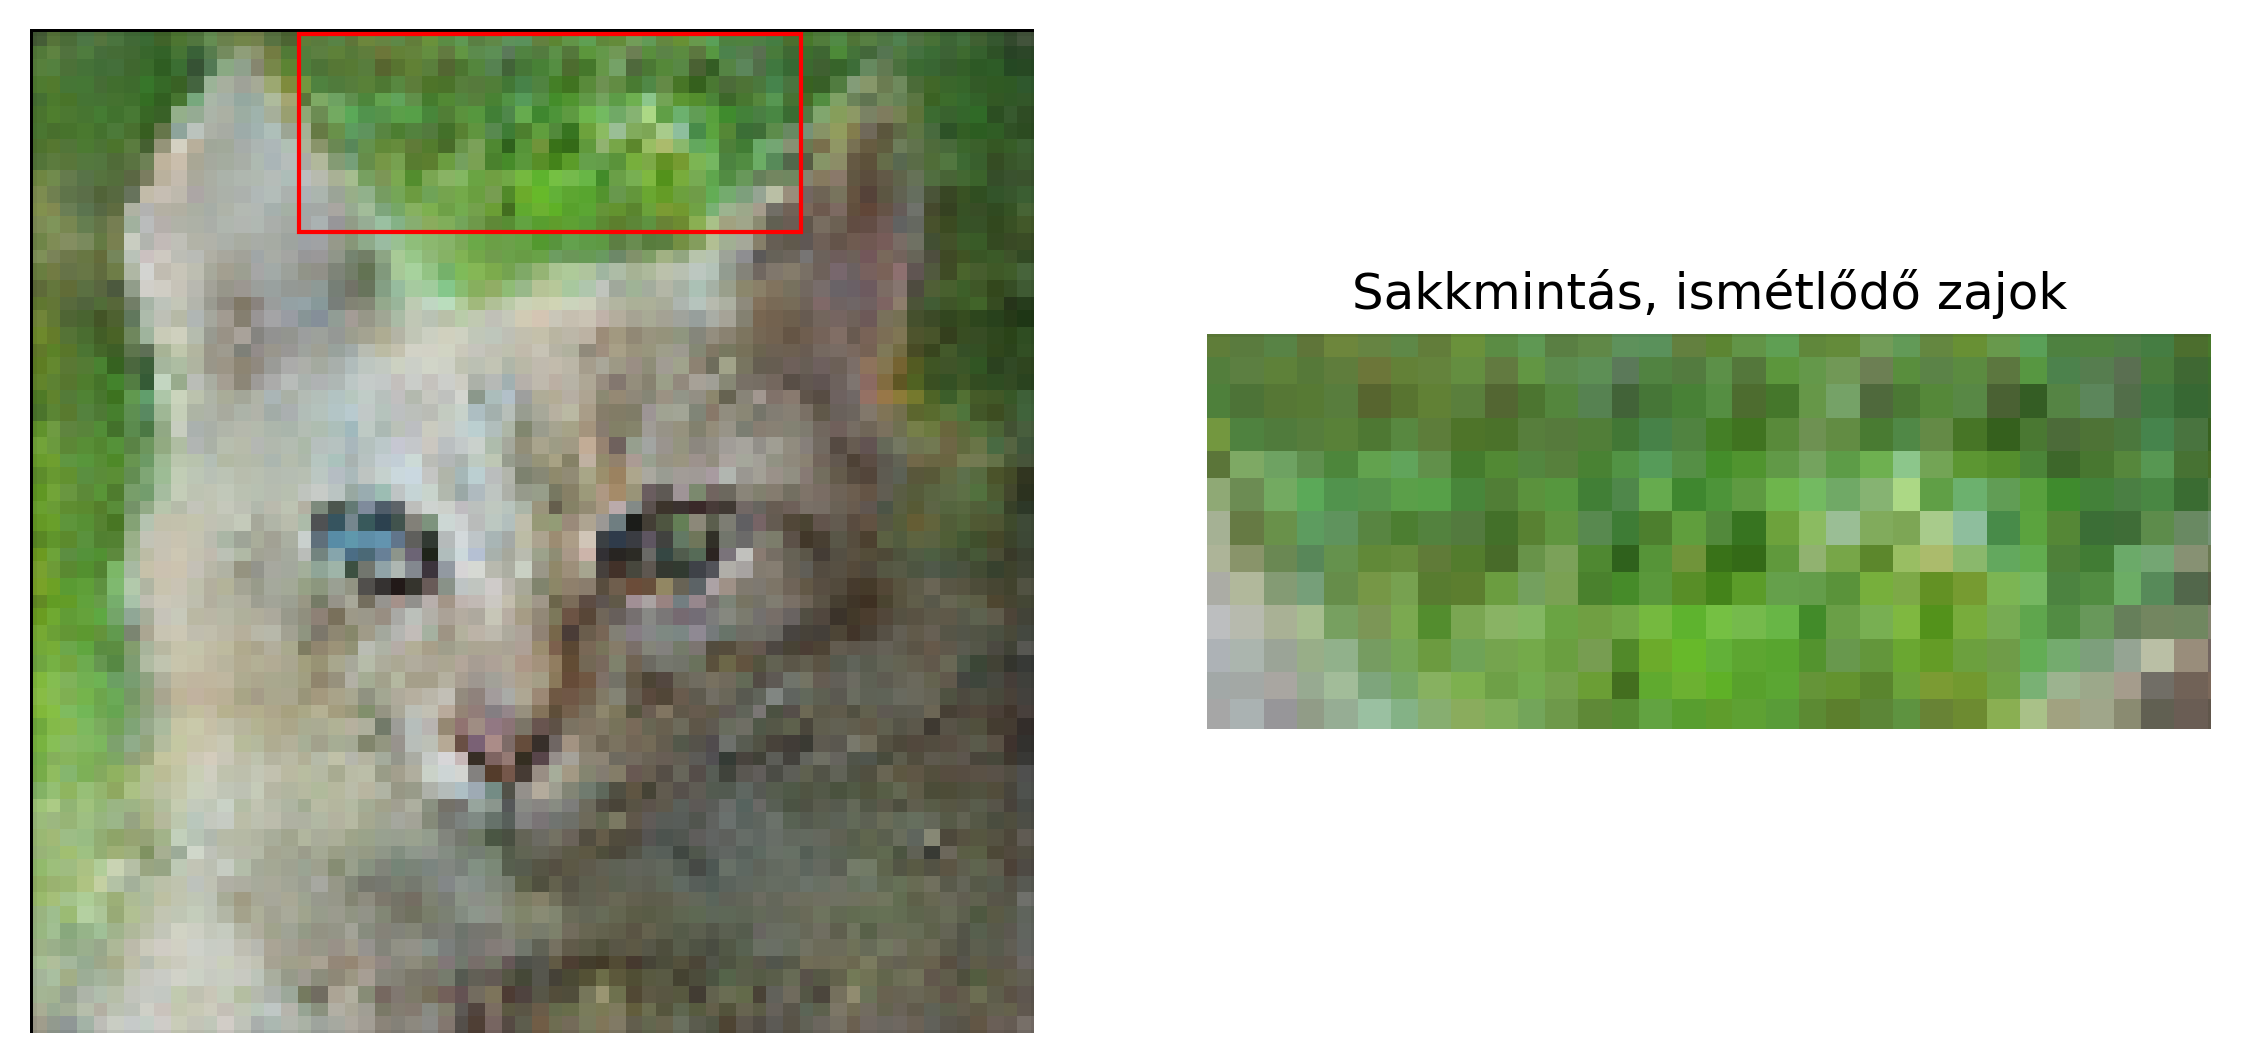
\includegraphics[width=13cm]{images/chessboard-patterns.png}
	\caption{Jellegzetes zajok a generált képeken}
	\label{fig:chessboard-patterns}
\end{figure}


\begin{itemize}
	\item A modell ebben a formájában igen hajlamos a \textit{mode collapse}-re, vagyis a tanulás során jelentkező összeomlásra. A jelenség és az elkerülésére irányuló néhány technika bemutatása a következőkben kerül ismertetésre.
	\item A konvolúciós rétegek működéséből adódóan csupán lokális pixel-környezetekre képes összefüggő részeket generálni a modell.\\
	Ez a működés alacsony felbontás mellett is anomáliákat idézhet elő, úgy mint a képeken megfigyelhető ismétlődő, sakktáblamintás zaj. Az említett zajra láthatunk példát \aref{fig:chessboard-patterns} ábrán. Megoldásként a Dekonvolúciós rétegek helyett a Konvolúciós és bilineáris interpolációval alkalmazott UpSampling rétegek használata javasolt \cite{odena2016deconvolution}.\\
	Ha a rejtett konvolúciós rétegek számával növelnénk a felbontást, akkor további nehézségbe is ütközünk: a modell nem lesz képes felismerni és megtanulni a tanítóminta képein megfigyelhető távoli, összefüggő tulajdonságokat. Így a generált képek részletezettsége alacsony lesz, gyakran \textit{blobokat} figyelhetünk meg csupán, különböző textúrákkal. \cite{salimans2016improved}
	
	\item A modellnek nincsen információja a különféle osztályokról, csupán a képek rendezetlen halmazán tanul, így magától kell megtanulnia a különféle osztályok jellegzetességeit.
	Az általánosítás szempontjából ez előnyös is lehet, viszont ha merőben különböző osztályokra szeretnénk betanítani a modellt, akkor az úgynevezett \textit{class conditoning} technika válhat a segítségünkre. A technikát a saját modellemre is kipróbáltam, a későbbiekben ismertetésre kerül.

\end{itemize}

\Section{GAN teljesítmény mérés}

A gépi tanulásos modellek tanítási életciklusának utolsó lépése optimális esetben a tesztelés. Hagyományos esetben a dataset-et három részre osztjuk fel: tanító-, teszt- és validáló halmazra. Hogy ezt milyen arányban tesszük meg, az függ a problémától is, de általánosan a teszt adathalmaz a dataset 20\%-a is lehet, a validáló halmaz még kisebb szelete a dataset-nek és a tanítóhalmazon történik a modell tanítása.
A teszt halmazt csupán egyetlen egyszer láthatja hagyományos esetben a modell, a tanítás után.
A teszthalmazzal szimuláljuk a modell valós adatokra történő alkalmazását, hiszen a modell számára ezen adatok teljesen ismeretlenek lesznek. A tesztadatok az eredeti dataset elemei, így rendelkezésünkre állnak az elvárt eredmények is, így a modell predikcióit össze tudjuk vetni az elvárt kimenettel, amelyből megbecsülhetjük a modell pontosságát különféle metrikák szerint.
A GAN esetében osztályozási feladatot a diszkriminátor lát el, viszont a hamis adatok nem részei a dataset-ünknek, azok a generátor által jöttek létre. A betanított modellnek csupán a generátora kerül felhasználásra, hiszen ezen komponens önmagában képes előállítani az új adatokat. A diszkriminátornak csupán a tanítás során van jelentősége és a validálásra önmagában nem alkalmas, hiszen ha a diszkriminátorunk rosszul tanult, úgy a generátorunk sem fog tudni a datasethez hasonló képeket generálni.
A GAN esetében nem szokás a dataset-et feldarabolni tanító és teszt részre, hiszen nem tudjuk a generátorra alkalmazni a már ismert metrikákat.
Ha képek generálása a feladat, úgy még nehezebb dolgunk van, hiszen a képeken hordozott információ igen összetett lehet.
A generátor kimenetét kell valamilyen módon tesztelnünk, ami nem egy egyértelmű feladat.
Egy emberi szemlélő természetesen meg tudná különböztetni a generált és a valós képeket. Lényegében a diszkriminátor feladatát látná el az emberi tesztelő, akinek hasonlóan mutathatnánk valódi és generált képeket, amelyekről el kell döntenie, hogy melyik a valódi és melyik a hamis. A fotórealisztikus képgenerálás igen nehéz feladat, és ha egy kicsit is rosszul teljesít a modell, azt egy emberi szemlélő hamar észreveszi és a modell pontossága igen alacsony lesz az emberi megfigyelő ítéletei alapján. Ha visszajelzést is kap az ember a hibáiról (Salimas et al. \cite{salimans2016improved}), akkor a továbbiakban sokkal pesszimistább ítéletet hoznak a tesztelők a képekre. Bináris, osztályozás helyett diszkrét vagy folytonos skálán is mérhetnénk a generált képeink jóságát. A pontos mérési eredmények érdekében több résztvevőt is be kellene vonnunk a tesztelésbe. Már belegondolva is igen lassú és költséges feladat lenne a modellünk tesztelése, így nem hagyatkozhatunk az emberi validálásra. Ez motiválta Salimas et al.-t is.

Az alábbi két ajánlás két mérőszámot definiál, amelyek segítségével meghatározhatjuk a GAN modellünk teljesítményét. Ezen validálási technikák megjelenése óta az újonnan megjelent GAN architektúrák mindegyikét lemérték és a GAN-al foglalkozó cikkekben táblázatokban vetik össze a különféle modellek teljesítményét a sajátjukkal.
A két mérőszámot együttesen szokták alkalmazni, hiszen egyik módszer sem tökéletes, viszont a kettőt együtt alkalmazva ad egy bizonyos képet a modellünk teljesítményéről.
A két mérőszám közös jellemzője, hogy mindkettő az Inception modell által kinyert jellegvektorok alapján határozza meg a modell jóságát.

Az alábbi kódrészlet az ImageNet adathalmazon betanított Inception modell használatát kívánja szemléltetni Keras segítségével. A kódrészlet első futtatásakor a modell súlyai letöltésre kerülnek és a további betöltés esetén egyből rendelkezésre fog állni.

\begin{python}
inception_model = keras.applications.InceptionV3(weights="imagenet")
predictions = inception_model.predict(images)
\end{python}

Az Inception modell bemenete alapértelmezett beállítások mellett egy $299 \times 299$ -es felbontású RGB színcsatornákkal rendelkező kép. A pixelértékeket normalizáltan várja a modell a $[-1, 1]$ tartományon. A modell inicializálásakor paraméterként megadhatjuk a bemenet méretét, viszont az nem lehet $75 \times 75$-nél kisebb. Ha az \texttt{include\_top} paramétert \texttt{True} értékkel állítjuk be, úgy a modell tartalmazni fogja az utolsó Dense rétegét is, amely az ImageNet súlyok alapján betanított modell esetében 1000 osztály detektálására lesz képes.

Az említett, GAN teljesítménymérésére használatos módszerek az \textit{Inception Score} (IS) és \textit{Fréchet Inception Distance} (FID). Ezeket kívánom bemutatni az alábbi két alfejezetben.

\SubSection{Inception Score}
Az Inception Score \cite{salimans2016improved} technikát Salimans et al. az emberi tesztelés kiváltására vetette fel. A méréseik alapján a technika sok minta figyelembevételével igen jól közelíti az emberi tesztelők által mért eredményeket.
Alapjául az Inception model szolgál, amelyet az ImageNet dataset-en tanítottak be. Minden egyes generált képet beadnak inputként a betanított Inception modellnek, hogy megkapják a conditional label eloszlást, ami tehát $p(y|x)$. Az olyan képeken, amelyeken jelentőségteljes objektumok figyelhetők meg, alacsony entrópiájú $p(y|x)$-el kell rendelkeznie. Vagyis a generált képen minél kevesebb objektumot kell felismernie a modellnek.
Továbbá az is lényeges szempont, hogy a generátor különféle képeket generálon, így a következőnek magas entrópiával kell rendelkeznie:
$$ \int \! p(y|x = G(z)) \; \mathrm{d}z. $$
Az Inception Score tehát:
$$ \exp(\mathbb{E}_x KL(p(y|x)||p(y))).$$
Minél magasabb ez a szám, annál jobbnak tekinthető a GAN teljesítménye.

Az Inception Score hivatalos implementációja\footnote{Az Inception Score hivatalos implementációja: \url{https://github.com/openai/improved-gan/tree/master/inception\_score}.} még a TensorFlow 1-es verziójában lett megírva, viszont a 2-es verzióval futtatva is működésre lehet bírni a megfelelő importok alkalmazása mellett. A méréshez a kigenerált képekre lesz szükségünk. A dolgozatom modelljeinek méréséhez a generált képek NumPy tömbökben kerültek kimentésre.

\SubSection{Fréchet Inception Distance}
Az Incepton Score kiegészítésére megjelent egy másik, széles körben elfogadott teljesítménymerő technika, a Fréchet Inception Distance (FID) \cite{heusel2017gans}. Az IS nem vette figyelembe a tanítóminta statisztikáit, és ez egy igen nagy hátránya a technikának. Továbbá az IS feltételein is javítottak, hogy a mintákon megtalálható zajok is befolyásolják a végső eredményt. Az FID számolásnál az Inception modell utolsó rejtett rétegének kimenetét veszik figyelembe, amely 2048 elemű jellegvektort jelent. A mérés elvégzése előtt a GAN modell tanításához használt adathalmazon kell vizsgálatot végezni, majd a generált képek kerülnek vizsgálatra, és az így kapott értékek alapján kapjuk meg a távolságot.

A számítási mód az alábbi formában adható meg:
$$ d^2((\boldsymbol{m}, \boldsymbol{C}), (\boldsymbol{m}_w, \boldsymbol{C}_w)) = \|\boldsymbol{m} - \boldsymbol{m}_w \|_2^2 + Tr(\boldsymbol{C} + \boldsymbol{C}_w - 2(\boldsymbol{C}\boldsymbol{C}_w)^{\frac{1}{2}}) $$
Minél alacsonyabb az FID, annál jobb a modell teljesítménye az adott tanítómintán.

Az FID hivatalos implementációja\footnote{A Fréchet Inception Distance hivatalos implementációja: \url{https://github.com/bioinf-jku/TTUR}.} szintén TensorFlow 1-ben került megvalósításra.

\Section{Mode collapse jelenség}

A \textit{Mode collapse} jelenség alatt a tanulás során bekövetkező azon anomáliát értjük, amely során a Generátor a látens tér bármely pontjára ugyanolyan kimeneti képet generál. A képek között minimális változatosság ugyan megfigyelhető, viszont a minőségük erősen romlik ilyen esetben. Előfordulhatnak olyan esetek is, amikor egy-egy megtanult képi jellegzetességek jelennek meg a kigenerált képeken teljesen indokolatlanul, és ezen jellegek helyére kerülnek újak a további tanítási lépések alatt. A tanítás közben felléphetnek lokális mode-collapse-ok is, amelyek a látens-tér egyes tartományaiban alakulhatnak ki \cite{zhang2018stackgan++}. \Aref{fig:mode-collapse}. ábrán láthatunk néhány példát a problémára.

\begin{figure}[h]
	\centering
	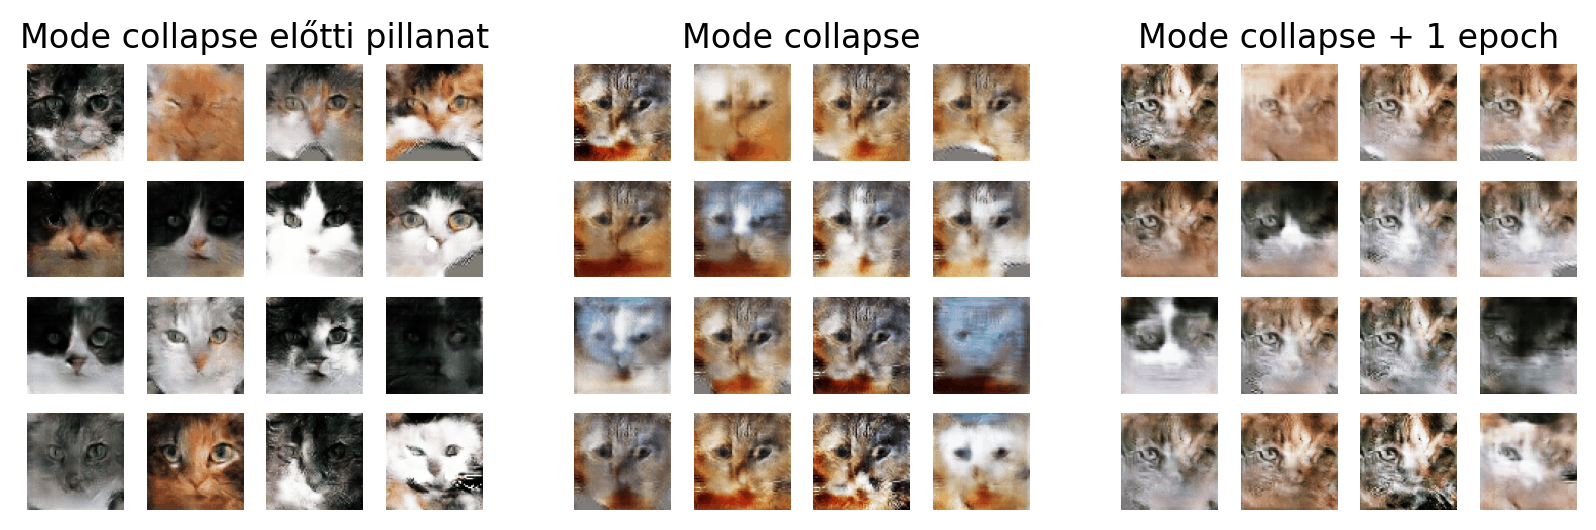
\includegraphics[width=15cm]{images/mode-collapse.png}
	\caption{Mode collapse jelensége}
	\label{fig:mode-collapse}
\end{figure}

Ez a jelenség valójában tekinthető egyfajta \textit{overfitting}-nek is, vagyis túltanulásnak, hiszen a Generátor úgy tudja átverni a Diszkriminátort, hogy közben a modell használhatatlan lesz. Viszont a mode-collapse elnevezés találóbb, hiszen amikor ez bekövetkezik, akkor a további tanítási lépések során úgy tűnhet, hogy stablinak tűnő modell hirtelen összeomlott volna.
A mode-collapse fellépése esetén a model további tanítása során minden egyes epoch-al változik a mode, vagyis az előzőtől eltérő kép jelenik meg a kimeneten (szintén minden egyes mintavételezett pontra hasonló). Mivel a diszkriminátor a mini-batch minden egyes bemenetét egymástól függetlenül dolgozza fel, így a gradienseiben sem jelenik meg olyan információ, amely a generátort változatosabb képek generálására bíztatná. A mode collapse esetén a diszkriminátor egyetlen pontot képes csak valódi adatnak tekinteni, majd minden egyes frissítéssel a pont elmozdul, ezzel magyarázható, hogy az összeomlás után tanítva minden egyes iterációval változik ezen pont, amire \textit{mode}-ként szokás hivatkozni \cite{salimans2016improved}. A GAN modellünk ezáltal használhatatlanná válik.

Egyes szerzők munkájában kiemelik, hogy az összeomlásig tanítják a felvázolt modelleket, és az összeomlás előtti állapotokra állítják vissza a hálózat súlyait a használathoz, mint például a BIG-GAN architektúra esetében is \cite{brock2018large}.

\begin{figure}[h]
	\centering
	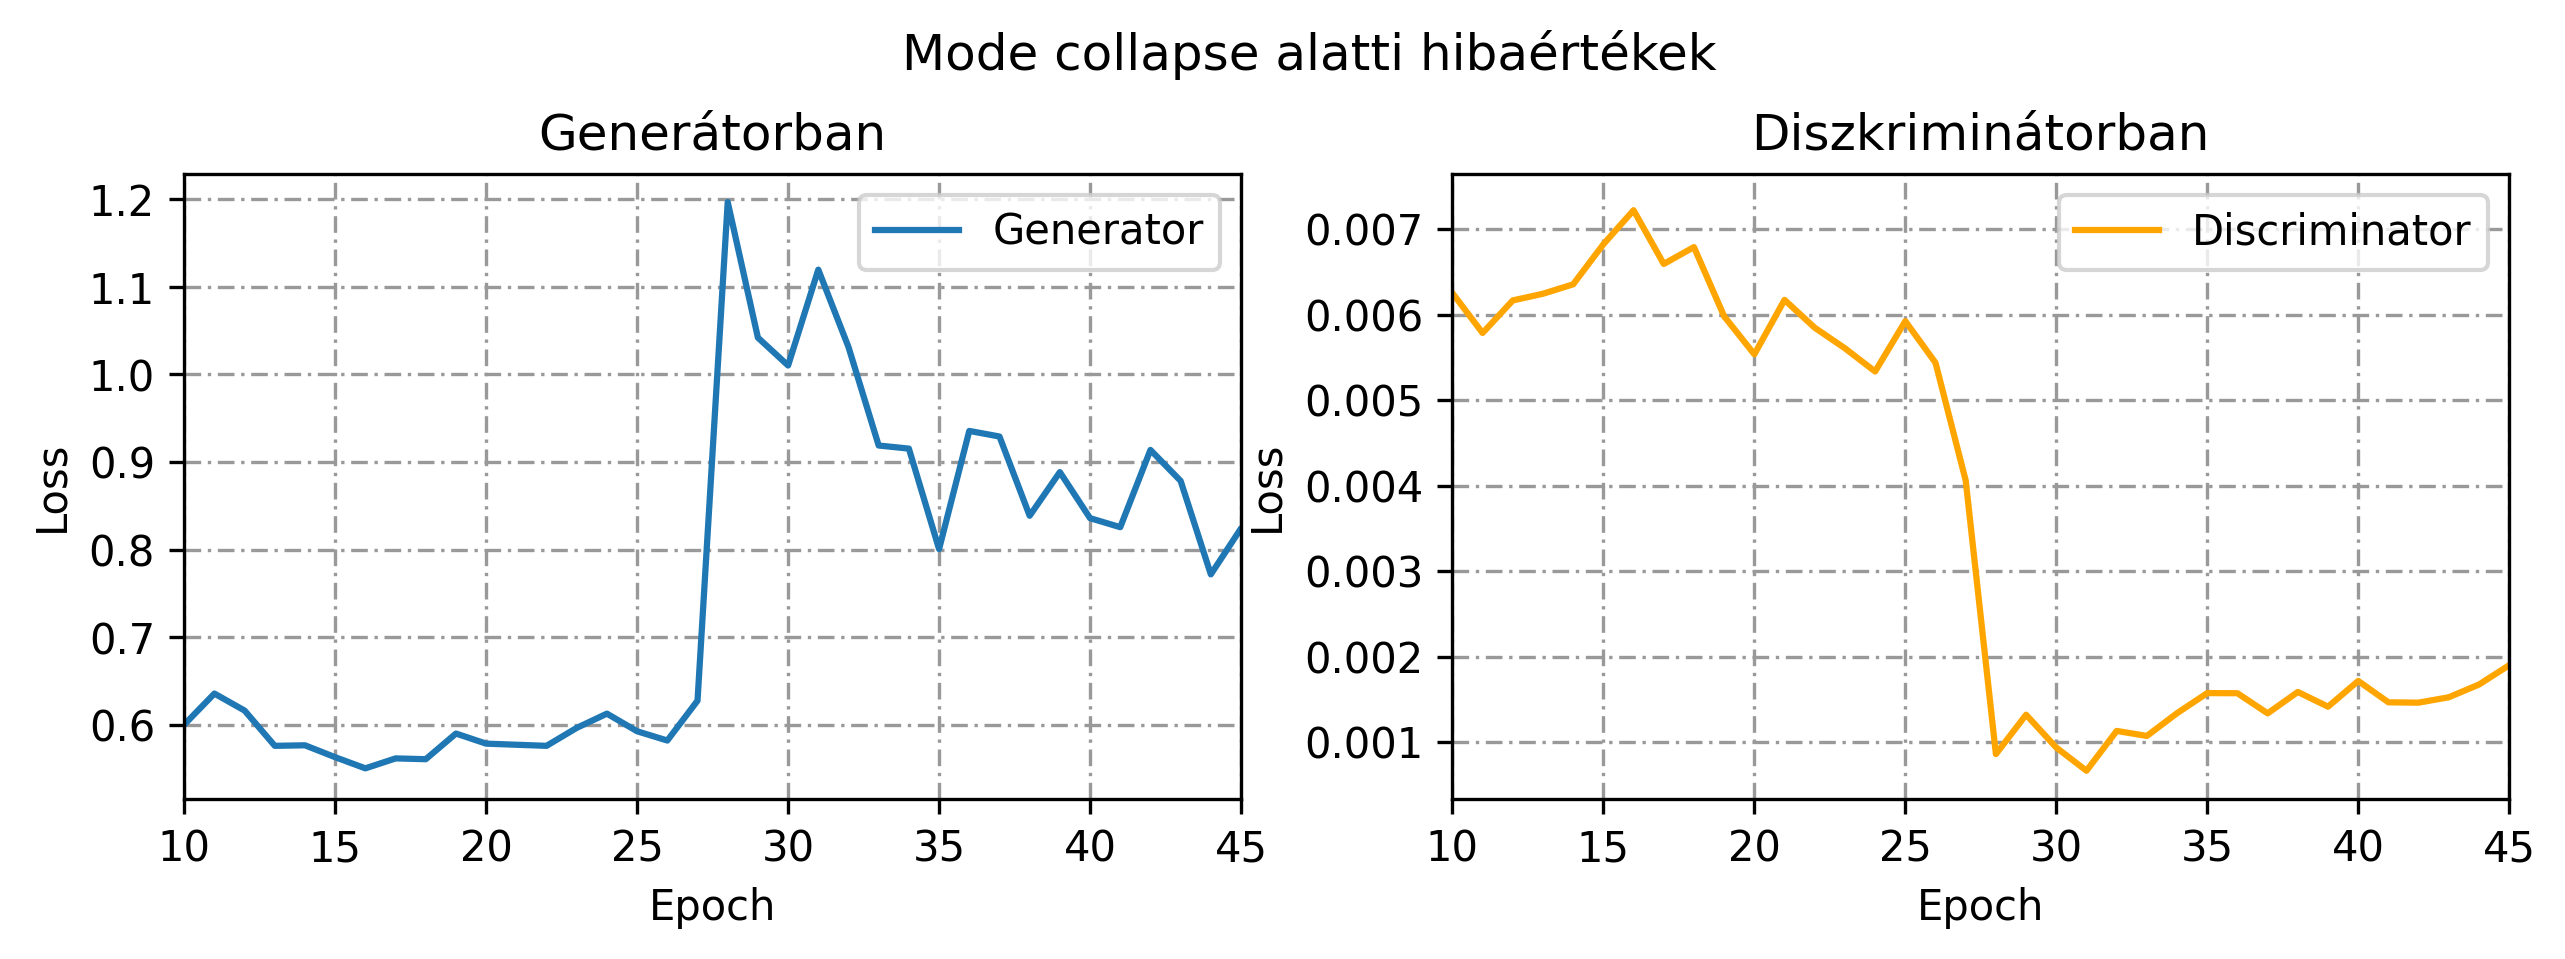
\includegraphics[width=15cm]{images/mode_collapse_loss.png}
	\caption{Mode collapse pillanata a hibagörbéken}
	\label{fig:mode_collapse_loss}
\end{figure}

\Aref{fig:mode_collapse_loss}. ábrán megfigyelhető a Generátor és a Diszkriminátor hibáinak alakulása a tanulás alatt. A kiugró hibaérték mindkét háló esetében ugyanazon epoch alatt jelentkeztek és a kimeneti képeket megvizsgálva megfigyelhetjük, hogy a modell valóban mode collapse áldozatává vált. Az ábrán azt is megfigyelhetjük, hogy a tanítás egészen korai szakaszában jelentkezett ezen anomália. Ennek oka az, hogy egy olyan adathalmazon tanítottam a modellt, amelyen semmiféle tisztítást nem alkalmaztak. Az adathalmaz a \textit{Flickr30k} \cite{young2014image}, amely egy ingyenes internetes képmegosztó weboldalról összegyűjtött képekből áll és 30 ezer képet tartalmaz. A képekhez leíró mondatok is tartoznak, amelyeket a tanítás során nem vettem figyelembe. Ilyen véletlenszerű és változatos képekre a modell jelenlegi formájában nem képes általánosítást találni, így a megfelelően előkészített adathalmaz továbbra is igen fontos része a GAN megfelelő tanításához.

A mode-collapse detektálása abban az esetben történhet a hibafüggvények vizsgálatával, ha a modellben teljes összeomlás figyelhető meg. A kisebb, lokális mode-collapse-ek esetében nem kapunk ilyen visszajelzést a hibafüggvényektől. A detektálásra alkalmasak lehetnek a validálási/teljesítménymérő módszerek is, vagyis az előbbiekben ismertetett IS és FID módszerek, amelyek a kigenerált képek változatosságát is figyelembe veszik az értékelés során.

\Section{Regularizációs módszerek}

A GAN tanítása során nehézségekbe ütközhetünk. Legrosszabb esetben nem is kezd el konvergálni a generátor kimenete a tanítóminta képeihez, viszont abban az esetben gyanakodhatunk, hogy a modellünk nem lett helyesen felépítve. Amennyiben mégis elkezd fejlődni a modell, és nem csak zaj jelenik meg a kimeneten az egyes tanítólépések után, de bizonyos számú epoch után mode collapse lép fel, úgy fontolóra vehetjük a következő regularizációs technikákat.

\SubSection{Label-smoothing}

A \textit{label-smoothing} az egyik legegyszerűbb regularizációs trükk, amely a neurális hálók overfitting problémáját kívánja kiküszöbölni. Ezen módszer alkalmazásához nem szükséges módosítanunk az architektúránkat, csupán a hibafüggvényt, így ez egy egészen egyszerűen implementálható technika. GAN esetében a diszkriminátor hibafüggvényét szokás módosítani oly módon, hogy a bináris keresztentrópia számolás során a valós bemeneti képek 1-es címke helyett valamennyivel alacsonyabb értéket, például 0.9-et kapnak. Ezzel a beállítással a diszkriminátor kevésbé lesz hajlamos a túlzott magabiztosságra a valós bemeneti képek esetén, teret adva a generátor fejlődésének. Ennek megvalósítása a következő Python kódrészletben látható.

\begin{python}
def discriminator_loss(real_output, fake_output):
    real_loss = cross_entropy(
    tf.constant(np.full(real_output.shape, 0.9)), real_output)
    fake_loss = cross_entropy(
    tf.constant(np.full(fake_output.shape, 0)), fake_output)
    total_loss = real_loss + fake_loss
    return total_loss
\end{python}

A regularizációs technikákban megfigyelhető néhány esetben egy kicsi ellentmondásosság is, például egyes technikák a diszkriminátort hátráltatják, míg mások a generátor dolgát nehezítik meg. Természetesen a problémától függ, hogy melyik módszer alkalmazható egy adott modellnél.


\SubSection{Megfelelő inicializációs stratégia}

A mély neurális hálózatoknál igen gyakran előforduló probléma az úgynevezett exploding vagy éppen a vanishing gradiensek jelensége, amelyet gyakran csupán instabil gradienseknek is szokás nevezni \cite{geron2019hands}.
A tanítás forward-propagation stádiumában a hálózat kimenetén megfigyelhető túl magas vagy éppen túl alacsony értékek a hibafüggvény meghatározásánál is szélsőséges értékeket okozhatnak.
A backpropagation stádiumában az output rétegtől haladunk az input felé, amely során kiszámolásra kerülnek a gradiensek a hálózat minden egyes paraméterének függvényében, majd Gradient Descent vagy ahhoz hasonló algoritmus segítségével frissülnek a hálózat paraméterei. Mindkét irányban fontos lenne elkerülni az esetleges kilengéseket, hogy a tanítás stabilitását elősegítsük.
Az olyan hálózatoknál, amelyekben több rejtett réteg is található, az instabil gradiensek jelensége még inkább érvényesül. A backpropagation során az input réteg felé haladva a gradiensek hajlamosak lehetnek igen kis értékekre zsugorodni. Ilyen esetben az alacsonyabb rétegek rendszerint lassabban fognak tanulni, amely szintén komoly problémát jelent.
A hálózat rétegeiben megtalálható neuronok az előző rétegek neuronjaitól függenek, illetve a kimenetük a következő réteg neuronjait is befolyásolja. Egy esetlegesen fellépő túl magas vagy túl alacsony kilengés a kimeneti értékekben komoly hatással lehet a teljes hálózatra.

Az instabil gradiensek megelőzésére az egyik irány a neuronok inicializációs stratégiájának megválasztása.
Az évek során több ajánlás is érkezett, a különböző felépítésű hálózatokra különböző technikák váltak be.

Kiemelnék két inicializációs technikát, a Glorot \cite{glorot2010understanding} és a He \cite{he2015delving} stratégiákat, amelyek széleskörűen alkalmazhatónak bizonyultak.
A kezdőértékek generálásához figyelembe veszik a rétegek be- és kimeneti kapcsolatainak számát is, amelyet $fan_{in}$ és $fan_{out}$-nak is nevezhetünk és azok átlagát használják fel a számoláshoz:
$$fan_{avg} = \frac{fan_{in} + fan_{out}}{2}.$$

A \textit{Glorot/Xavier} inicializációs stratégia normális és egyenletes eloszlásra is számolható.
Normális eloszlás esetén a várható értéket $m = 0$-ra kell választani, a szórásnégyzet pedig: $ \sigma^2 = \frac{1}{fan_{avg}} $, tehát
$$ \mathcal{N}\left(0, \frac{1}{fan_{avg}}\right). $$
Egyenletes eloszlás esetén $\pm r$ között (vagyis $ \mathcal{U}\left[-r, r\right] $):
$$r = \sqrt{\frac{3}{fan_{avg}}}.$$

Ezen inicializációs stratégia a tangens-hiperbolikusz, logisztikus és softmax aktivációs függvényekkel rendelkező rétegekben használatosak. 

A \textit{He/Kaiming} inicializáció hasonló megközelítést alkalmaz.
Normális eloszlásra:
$$ \mathcal{N}\left(0, \frac{2}{fan_{in}}\right), $$
Egyenletes eloszlásra ($ \mathcal{U}\left[-r, r\right] $):
$$r = \sqrt{3 \cdot \frac{2}{fan_{in}}}.$$

Ezen inicializációs stratégia pedig a ReLU aktivációs függvények családjával rendelkező rétegekben ajánlott használni.

A Keras a Glorot inicializálást használja alapértelmezetten.

\SubSection{Batch Normalization}

Az instabil gradiensek problémája a tanítás során is jelentkezhet. A megfelelő inicializációs stratégia nem garantálja a teljes stabilitást, csupán egy kezdeti optimális állapotot biztosít a modellnek.
Az input adatok standardizálása áll a Batch Normalization technika mögött, amelyet a rétegek között vagy a rétegek aktivációs függvénye előtt ajánlott megtenni. A Batch Normalization technika alkalmazásához tehát minimálisan módosítanunk kell a meglévő modelljeink architektúráját. Azt figyeltem meg, hogy ezen technika alkalmazása teljesen empirikus módon történik és nincsen egy általánosan elfogadott módszer arra sem, hogy pontosan hol kell elhelyezni a réteget: az aktivációs függvények előtt vagy után. Kétségtelen, hogy a technika alkalmazásával stabilabb tanítást eredményez és széleskörűen alkalmazható a mély neurális hálózatokban.

A Batch Normalization technika 0 közepűvé teszi és normalizálja az inputokat, majd skálázza és shifteli az eredményeket. Vagyis két tanulható paramétervektor jelenik meg rétegenként a modellünkben, a skálázás és a shiftelés műveletre. A technika neve a mini-batch tanítási stratégiából adódik, vagyis amikor egy tanítási lépést nem a teljes dataset-re hajtunk végre, csupán annak egy kisebb szeletére. A Batch Normalization zero-centerező és normalizáló lépéséhez az algoritmusnak meg kell becsülnie az aktuális bemeneti mini-batch várható értékét és szórását. Ezt a becslést csupán tanítási időben tudja megtenni az algoritmus, hiszen olyankor rendelkezésére áll a teljes mini-batch. Viszont tesztelésnél, amikor csupán egy-egy tesztadatot lát a modell, úgy nem hagyatkozhatunk a becsült várhatóértékre és szórásra. A Keras-ban található implementáció a tanulás során mozgóátlaggal vezeti a várhatóértékeket és a szórásokat. Ez további két paramétert jelent, amelyeket a modell a tanulási folyamat során fog meghatározni a már említett módon, viszont a backpropagation során nem kerülnek finomhangolásra, csupán tesztidőben használja ezeket az értékeket.

Az algoritmus működése a következőképpen írható fel \cite{geron2019hands}:

Legyen $m$ a mini-batch elemszáma, $m \in \mathbb{N}, 0 < m \leq n$, ahol $n$ a dataset elemszáma, a minta pedig $X = \{x_1, x_2, \ldots, x_m \}$. 

1. Határozzuk meg a várható értékeket a mini-batch elemeire
$$ \mu = \frac{1}{m} \sum_{i=1}^{m} x_i. $$

2. Határozzuk meg a szórásnégyzeteket a mini-batch elemeire:
$$ \sigma^2 = \frac{1}{m} \sum_{i=1}^{m} (x_i - \mu)^2. $$

3. Zero-centerezzük és normalizáljuk az inputokat. $\varepsilon$ egy kicsi szám (általában $10^{-5}$), ami a 0-val való osztás elkerülése érdekében van jelen:
$$ \hat{x_i} = \frac{x_i - \mu}{\sqrt{\sigma^2 + \varepsilon}}. $$

4. Skálázzuk a $\gamma$ és shifteljük $\beta$ paraméterekkel az inputokat
$$ z_i = \gamma \otimes \hat{x_i} + \beta$$

Az algoritmus kimenete a $z_i$.


\SubSection{Two Time-Scale Update Rule (TTUR)}
Ezen technikát szintén meg lehet valósítani architektúrális változtatás nélkül, csupán az Adam optimalizáló eljárás egyik paraméterét kell megfelelően beállítani az implementációjához.
Heusel et al. \cite{heusel2017gans} cikkében mérésekkel alátámasztották, hogy ha az Adam optimalizáló módszert választjuk a GAN tanításához és a learning rate paramétert a Generátorban és a Diszkriminátorban különbözőre állítjuk, úgy a modell gyorsabban és stabilabban fog konvergálni a lokális optimumokhoz.
Például a Generátor optimalizálójában a 0.0001-es tanulási mérték és a Diszkriminátor optimalizálójában beállított 0.0004 érték ezt a technikát valósítja meg.

A bemutatott regularizációs technikák csupán a legismertebbek. Az egyéb módszereket nem sikerült megfelelően alkalmaznom, így nem kerülnek említésre.

\Section{A képgeneráló modell kibővítési lehetőségei}

A felvázolt GAN architektúra  alapként szolgálhat különféle háló típusokhoz. Az irodalomkutatás során talált megoldásokban is megfigyelhető, hogy jellemzően mély-konvolúciós szerkezeten alapuló megoldásokat alkalmaznak különféle kiegészítésekkel. A jobb eredmény érdekében igen szerteágazó kiegészítési javaslatok jelentek meg. Ezen alfejezetben két kibővítési lehetőség kerül ismertetésere.

\SubSection{Tanítás címkékkel}

A GAN alap esetben minták rendezetlen halmazán tanul. Viszont a legtöbb adathalmaz annotációkkal van ellátva, amelyeket így nem veszünk figyelembe a tanítás során, és a modellre bízzuk, hogy megtanulja reprezentálni a tanítóhalmaz különféle objektumait. Ha szempont, hogy a GAN különféle osztályokra tudjon képeket generálni, akkor használhatjuk a \textit{Class Conditioning} technikát \cite{mirza2014conditional}. Ezen technika alkalmazása mellett a modellnek egyfajta könnyítést is adhatunk a tanulás során, ha olyan adathalmazra végezzük el a tanítást, amely többfajta osztály objektumait tartalmazza. A technika alkalmazásával a modellünk nem a teljes adathalmazra próbál általánosítást találni, csupán az egyes osztályokra. Így azt feltételezhetjük, hogy az osztályok tudatában könnyebben tud majd tanulni.

A class-conditioning technika alkalmazása során a Generátor és a Diszkriminátor egyszerre kerül kondícionálásra, vagyis minden egyes tanítási lépésnél a kondicionáló címkék meg fognak egyezni. Viszont a tanítás során nem ellenőrizzük le, hogy valóban helyesen lettek-e kondicionálva, hiszen továbbra is a megszokott kimenetekkel fog rendelkezni a Generátor és a Diszkriminátor is.

A hibafüggvény a következőképpen írható fel:
$$\min_{G}\max_{D}V(D, G) =  \mathbb{E}_{x \sim P(x)} \left[\ln D(x|y) \right] + \mathbb{E}_{z \sim P(z)} \left[\ln(1 - D(G(z|y))) \right].$$

Egy-egy tanítási lépés során a Generátor és a Diszkriminátor is ugyan azt az $y$ címkét kapja bemenetként (pontosabban a Diszkriminátor az $y$ címkéhez tartozó valós képeket). A kondícionálás lényegében csupán annyit jelent, hogy az egyes tanítási lépések során hasonló bemenetet kap a két modell és ezen bemenetet hasonlóan dolgozzák fel.

Az architektúrát mindkét oldalon módosítani kell a technika megvalósításához. Az eredeti cikkben \cite{mirza2014conditional} kiemelték, hogy a $P(z)$ zajvektor és az $y$ címke kombinálására vonatkozólag a GAN keretrendszer igen rugalmas tud lenni. A rugalmasság a kombinálásra is vonatkozhat, vagyis a szerzők nem is kötötték meg, hogy milyen módon lehet összeilleszteni a $z$-t és $y$-t. Én az egyszerűség kedvéért egy \textit{multiply} réteget választottam, hiszen így nem változik a bemeneti dimenziószám, és a kondicionálást a Generátor elején el lehet végezni. Viszont meg lehet fontolni több komponáló módot is, mint például a konkatenációt, vagy az \textit{add} réteg használatát is. További vizsgálatokat nem végeztem ez irányban.

Az $y$ címke a Cifar-10 adathalmaz esetében egy egész szám, amely 0 és 9 közötti értéket vehet fel. Az $y$ címkét egy \textit{embedding} réteg segítségével egy, a látens dimenzióval megegyező vektorrá alakítjuk, majd a $z$ zajvektorral való összeszorzás előtt egy \textit{flatten} réteggel a megfelelő formára hozzuk a kimeneti tenzort.
A \textit{multiply} réteg segítségével összeszorzásra kerül az vektorizált címke és a zajvektor, amelynek kimenete lesz a Generátor modellünk bemenete (\ref{fig:labelnoiseembedding}. ábra). A Generátor modell felépítése megegyezik a már ismert, korábban felvázolt Generátor architektúrájával.

\begin{figure}[h]
	\centering
	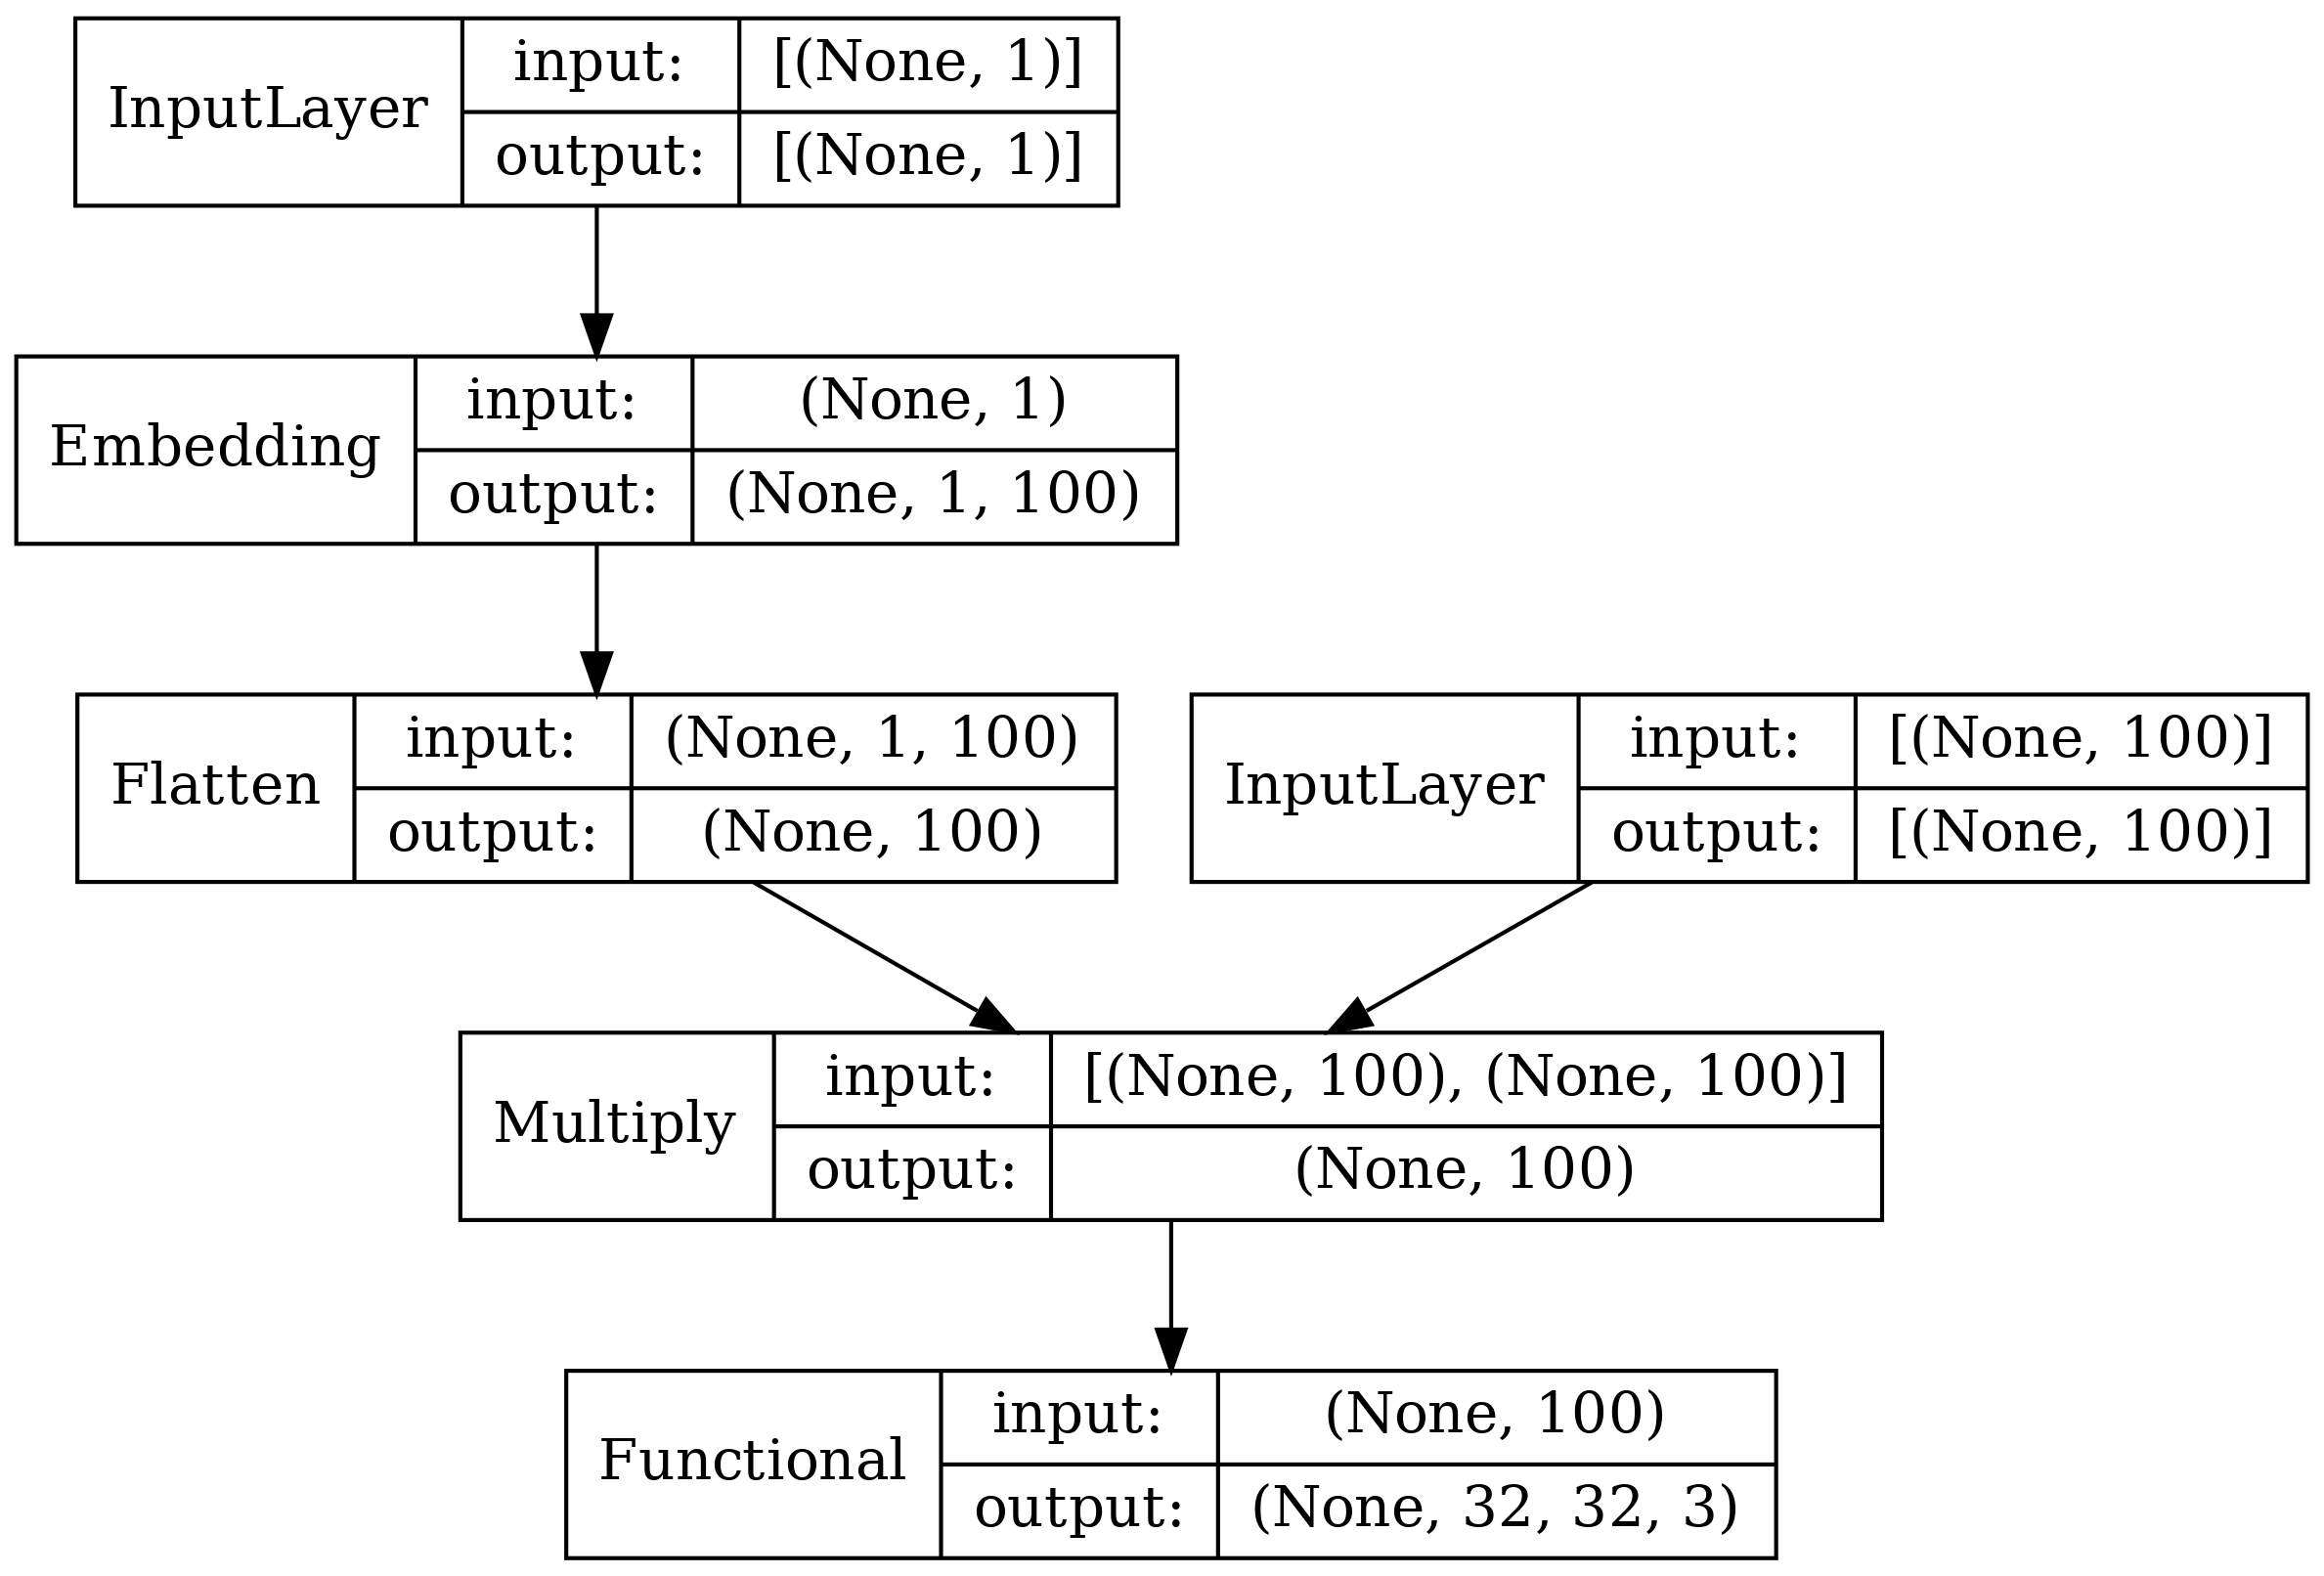
\includegraphics[width=10cm]{images/label_noise_embedding.png}
	\caption{A zajvektor és a címke összeállítása a generátor bemeneteként}
	\label{fig:labelnoiseembedding}
\end{figure}

A Diszkriminátorban a kondicionálást a modell belsejében hajtom végre. Mivel a Diszkriminátorunk a Generátor tükörképének is tekinthető, így a Diszkriminátor esetén nem a képpel együtt kerül be a címke a modellbe, hanem a modell által kinyert belső reprezentációkkal kerül összeszorzásra a címkét reprezentáló vektor, az utolsó teljesen összekapcsolt réteg előtt. A label conditioning technikát felvető cikkben megemlítették a \textit{dropout} réteg használatát is, így a teljesen összekapcsolt réteg előtt beillesztettem egy olyan réteget is.
A Diszkriminátor felépítése \aref{fig:labeldiscriminator}. ábrán figyelhető meg.

\begin{figure}[h]
	\centering
	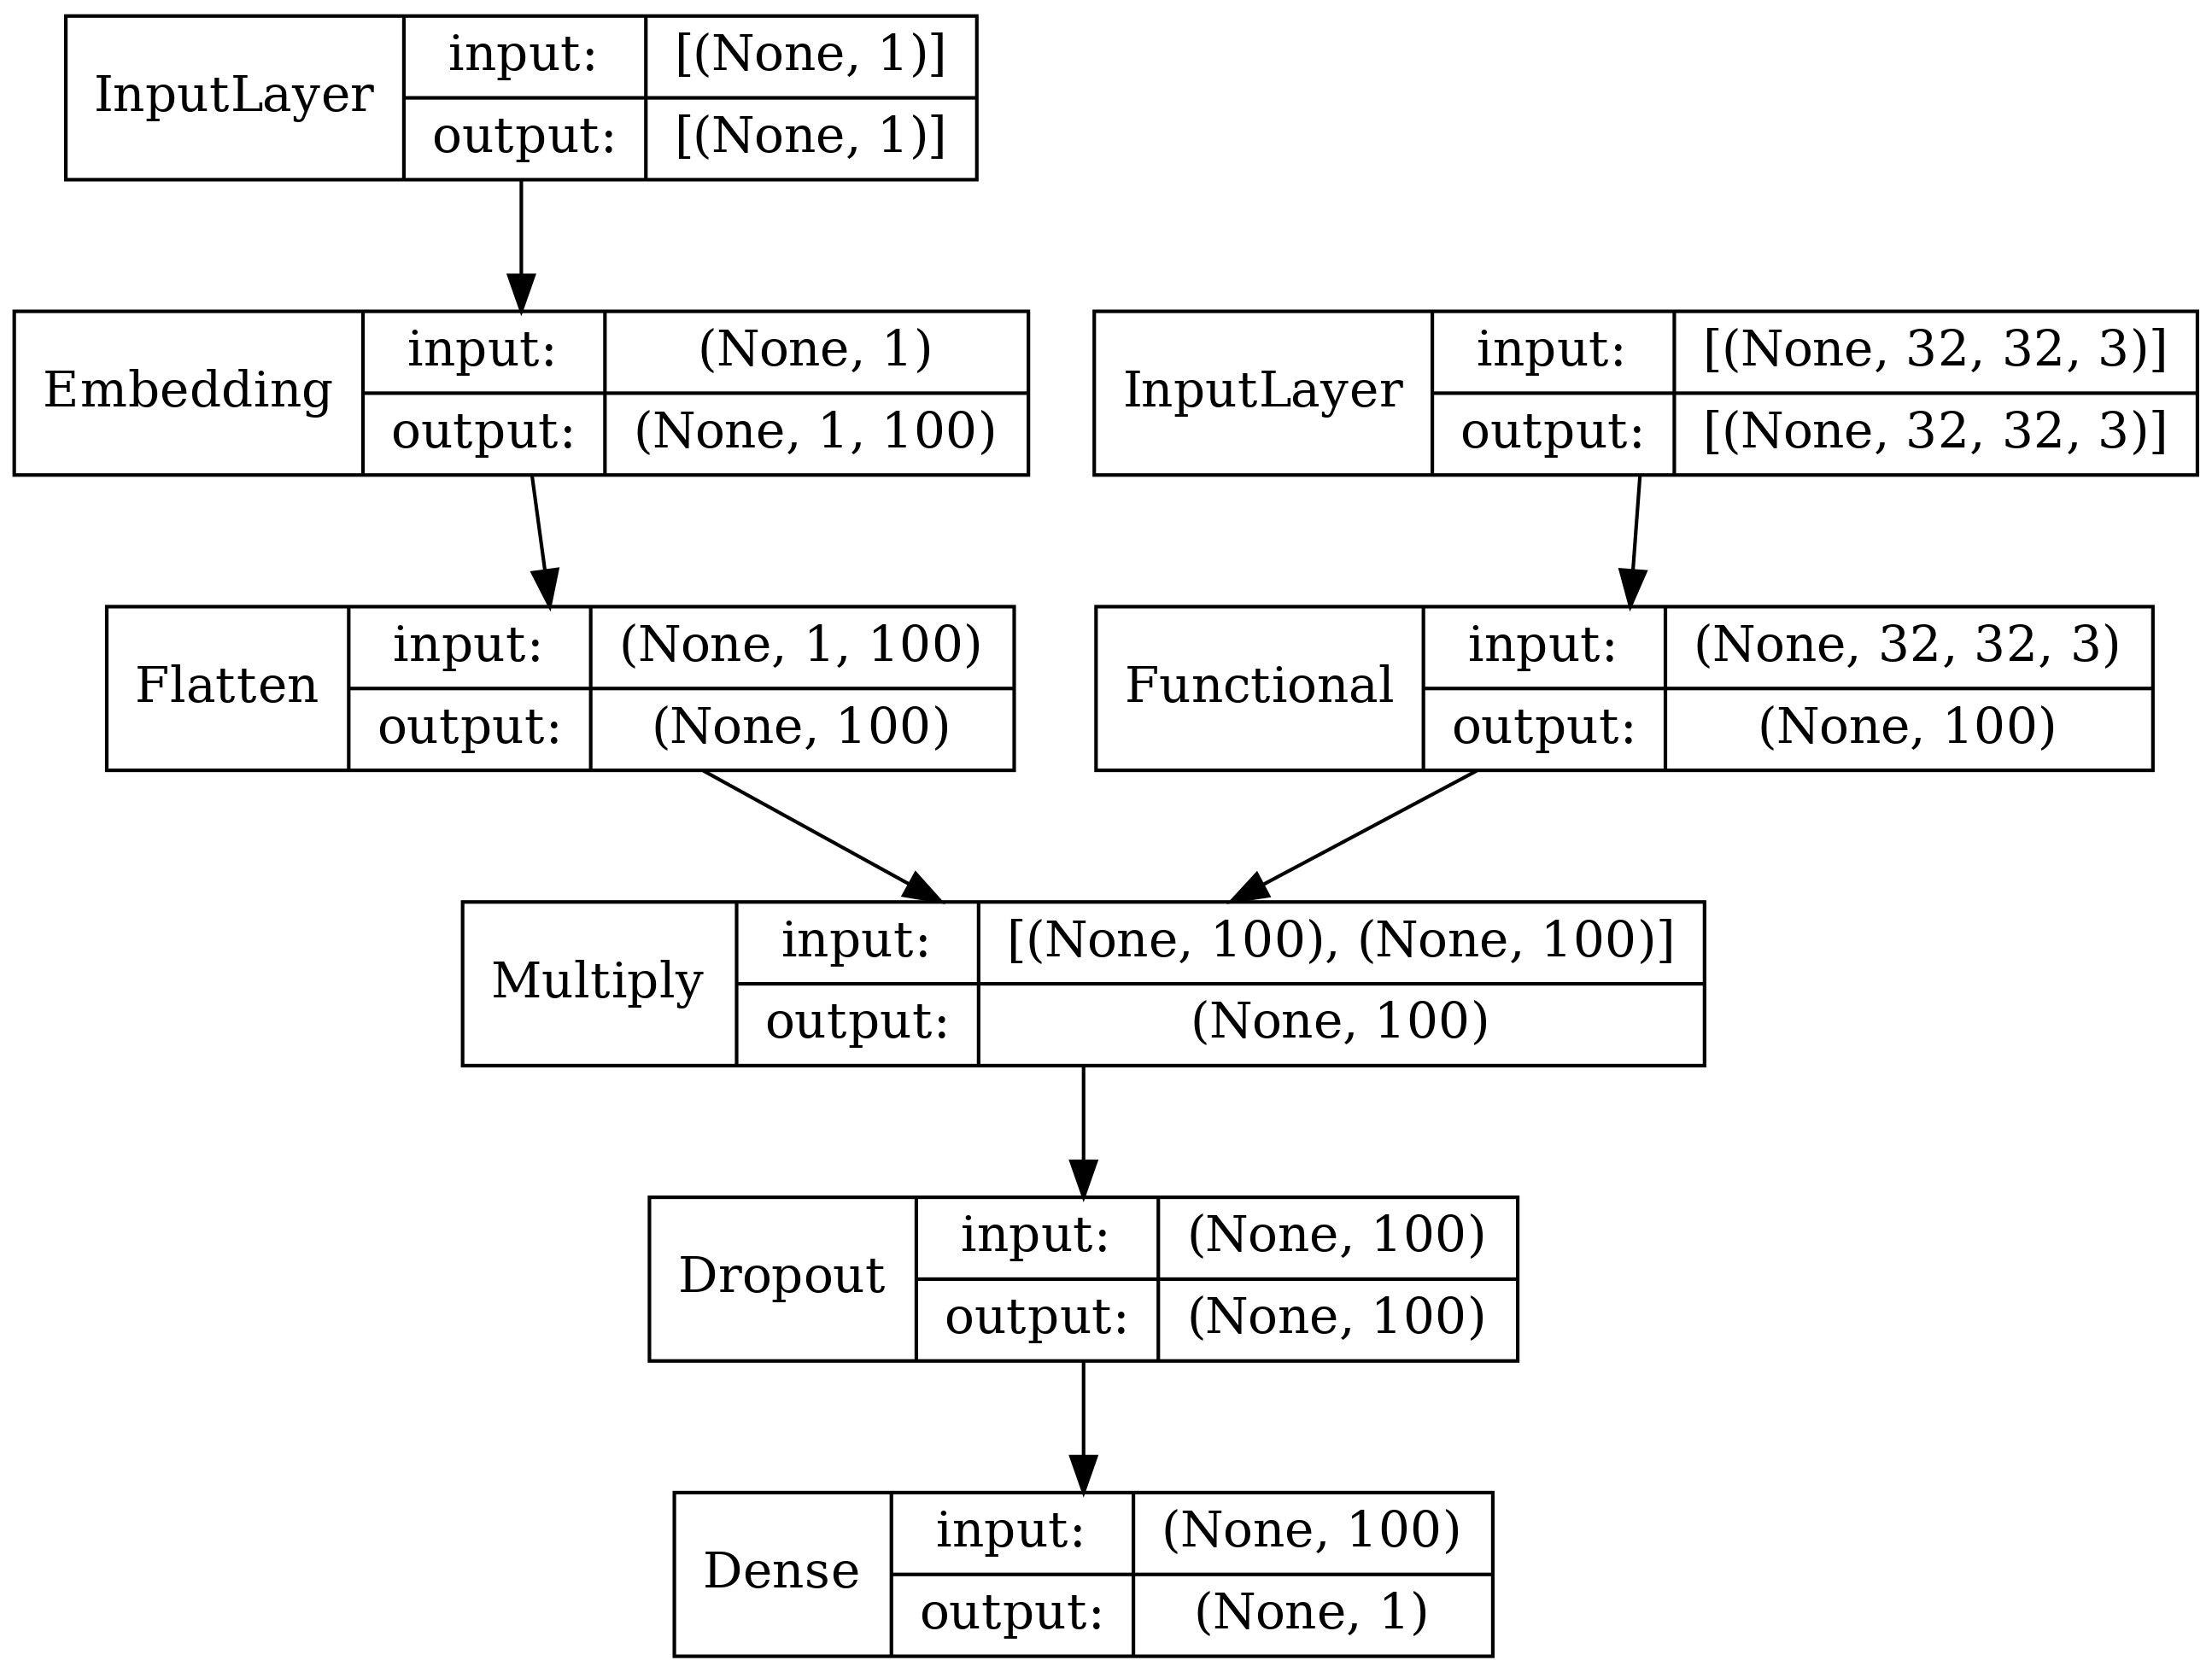
\includegraphics[width=10cm]{images/label_discriminator.png}
	\caption{A belső reprezentá és a címke összeállítása a diszkriminátorban}
	\label{fig:labeldiscriminator}
\end{figure}

A betanított háló kimeneteire példát \aref{fig:labelconditioning}. ábrán láthatunk, amely a már említett Cifar-10 adathalmaz 10 darab osztályára tanult be. A tanítás során megfigyeltem, hogy az osztályokon belül jelentkezik a mode-collapse jelensége, amely a regularizációs technikák alkalmazása mellett valamelyest javítható, viszont nem sikerült úgy betanítani a modellt, hogy igazán változatos képeket generáljon. A bemeneti zajvektor dimenziójának növelésével is némileg később jelentezett a mode-collapse, viszont egy ilyen kisebb példánál, $32 \times 32$-es felbontás mellett nem indokolt az 512 dimenziójú zajvektor használata, így ez nem tekinthető megoldásnak a mode-collapse-re, hiszen a modellek paramétereinek száma is megnövekedett a GAN-ban.
A technika másik hátránya, hogy az osztályok között igen éles határ alakul ki, vagyis nem lehet olyan bemeneti címkét megadni, aminek hatására kevert osztályokat is ki tudna generálni a modell. Minden esetben csupán egyetlen osztály képének megalkotására képes, még akkor is, ha nem egész értékeket adunk meg címkének. Két címke között interpolálva egyszerűen az egyik határponton átugrik a modell kimenete a következő címkének a kimenetére.

A tanítás kiegyensúlyozatlansága, és a kevert osztályok reprezentálásának hiánya miatt úgy gondoltam, hogy nem ezen megoldás lesz számomra a legkedvezőbb.

\begin{figure}[h]
	\centering
	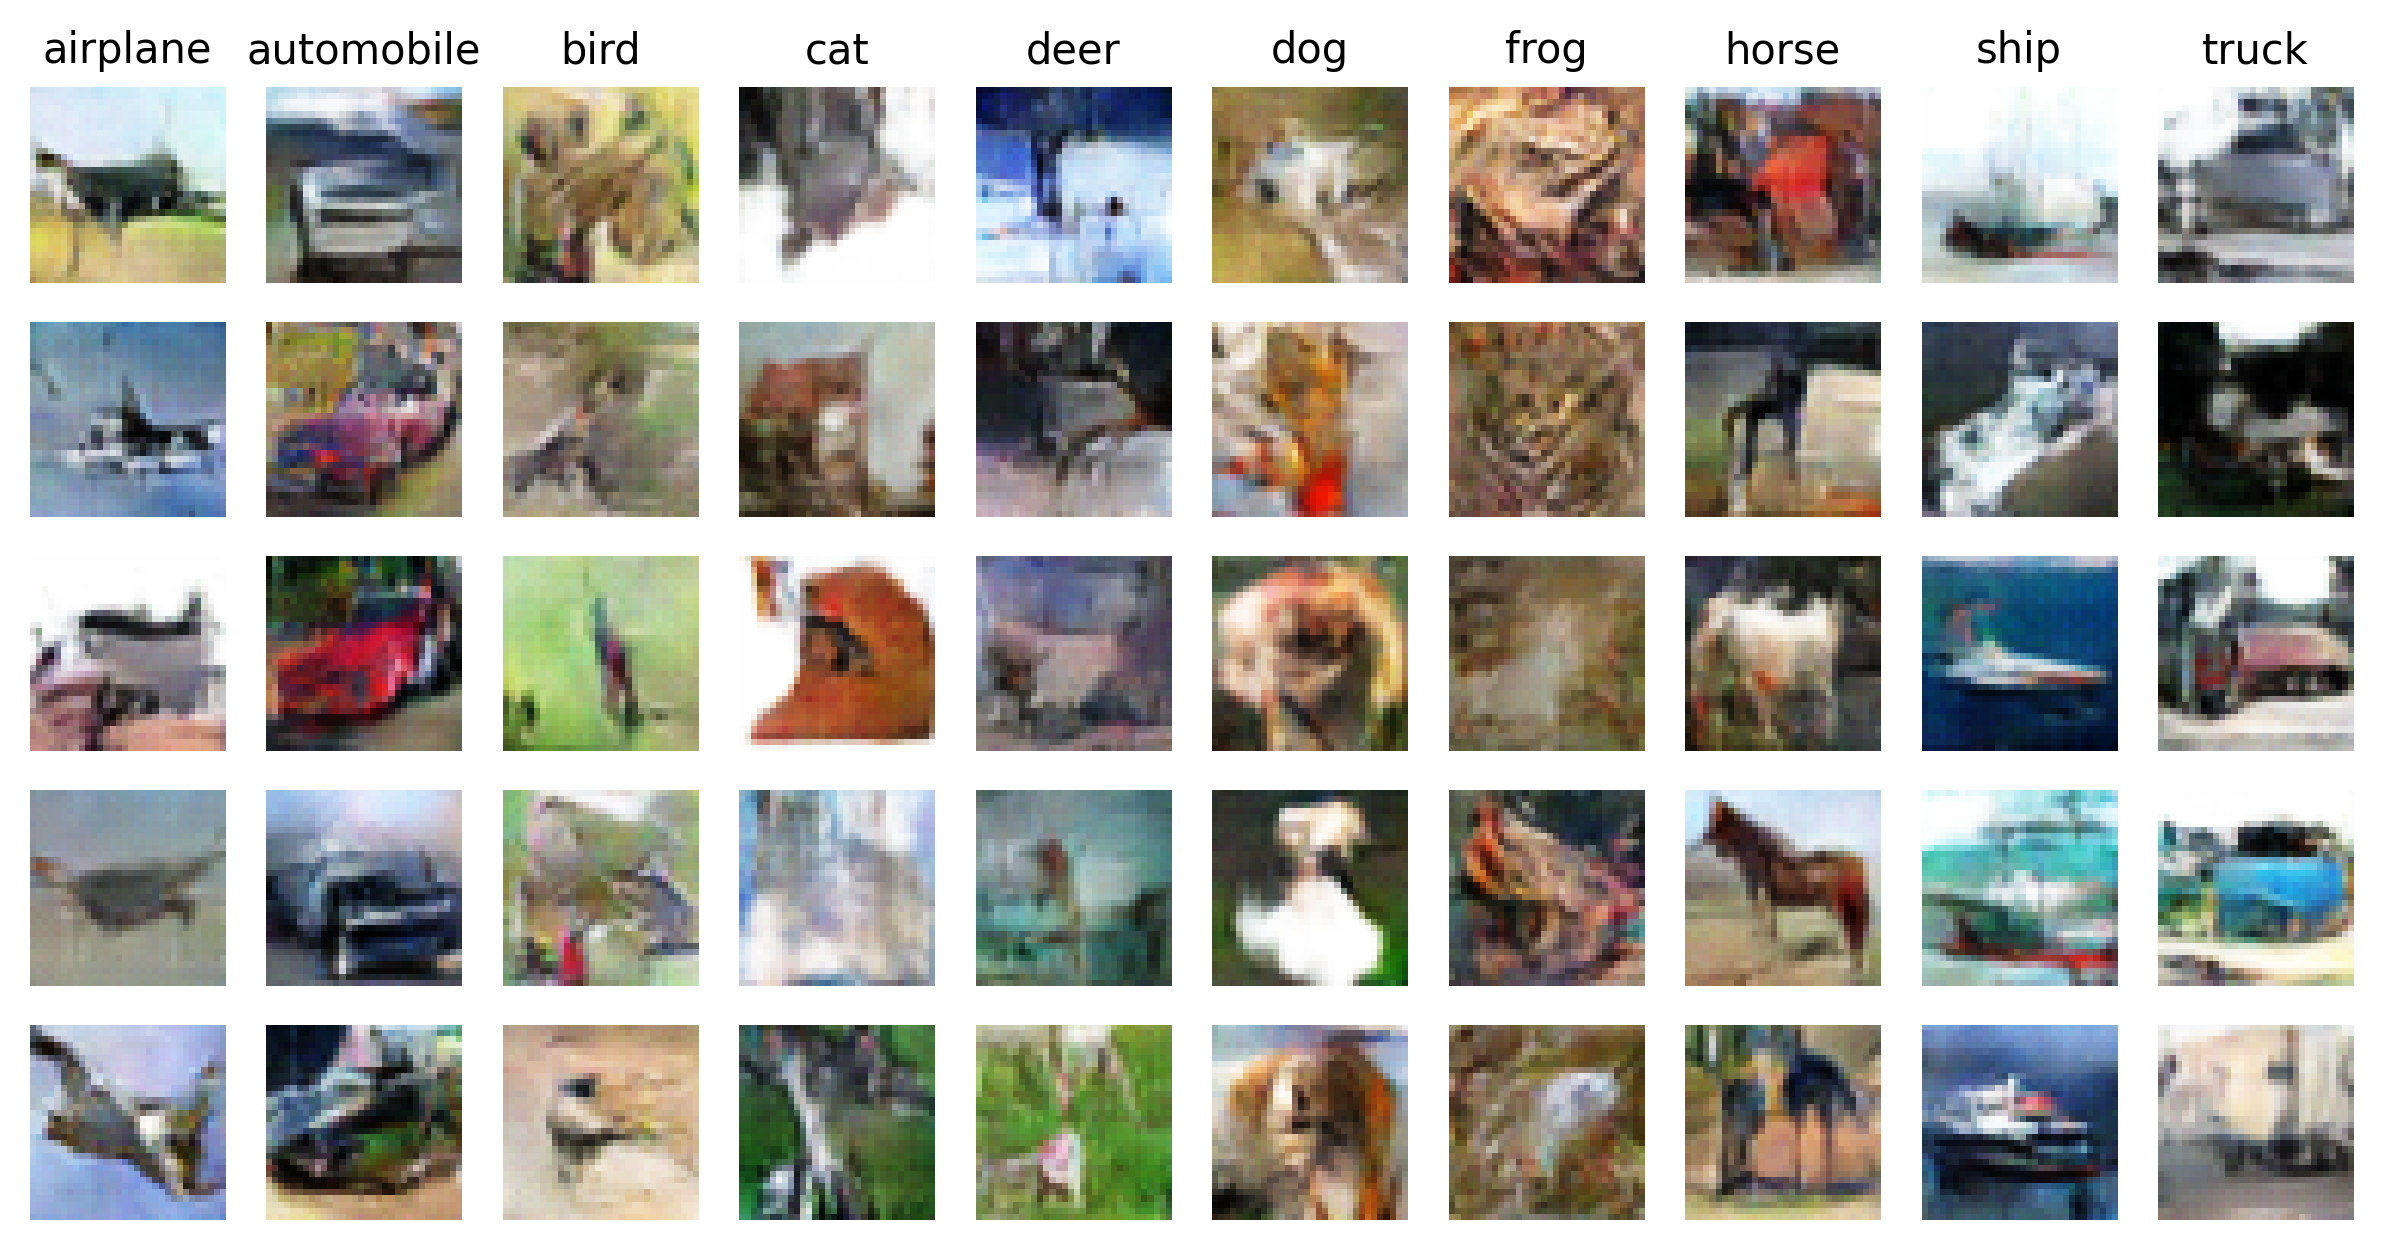
\includegraphics[width=13cm]{images/label_conditioning.png}
	\caption{Label conditioning technikával tanított Generátor kimenetei}
	\label{fig:labelconditioning}
\end{figure}

\SubSection{Multi-Scale Gradient architektúra}

Egy másik kiegészítésként a \textit{Multi-Scale Gradient} (MSG) alapján több ki- és bemenettel láttam el a Generátort és a Diszkriminátort \cite{karnewar2020msg}. Igyekeztem az eredeti modellemet kiegészíteni és alkalmazni az MSG-ben látottakat, vagyis az U-net szerű kapcsolatokat. Ugyan a \textit{Multi-Scale Gradient} architektúra implementálása nem hozta el az architektúrához publikált eredményeket, viszont a kigenerált képek minőségét valamelyest javította. Az eredeti és ezen modell eredményeinek összehasonlítására az alfejezet végén láthatunk majd összehasonlítást.

A kibővített modell Generátora összességében megegyezik az eredeti modellel, csupán több kimenettel rendelkezik. A belső rétegekben található reprezentációkból egy-egy konvolúciós réteg segítségével állítja elő a modell a kimeneteket. A korábban említett \textit{toRGB} rétegnek felelnek meg ezek a rétegek. Az aktivációs függvénye ezen rétegeknek a tangens hiperbolikusz, hasonlóan az eredeti modell utolsó rétegéhez.
A Generátorba került még minden dekonvolúciós réteg után egy-egy \textit{BatchNormalization} réteg is, továbbá alkalmazásra került a He-féle inicializálási stratégia is.
A saját implementációmban a \textit{toRGB} konvolúciós réteg a következő táblázatban megfigyelhető paraméterekkel lett ellátva:

\small{
\begin{center}
\begin{tabular}{@{\extracolsep{6pt}} c c c c c }
	\hline
	\multicolumn{5}{l}{\textbf{\textit{toRGB} konvolúciós réteg}} \\
	\hline
	Filterek száma & Kernelméret & Strides & Padding & Aktivációs függvény\\
	\cline{1-1} \cline{2-2} \cline{3-3} \cline{4-4} \cline{5-5}
	3 db & $4 \times 4$ & $1 \times 1$ & "same" & tangens hiperbolikusz\\
	\hline
\end{tabular}
\end{center}
}

A 4 darab \textit{toRGB} réteg további 46092 darab hiper-paramétert jelent, amelyek a tanítás során kerülnek finomhangolásra. Az eredeti modell milliós hiper-paraméter nagysága mellett nem tűnik olyan nagy kiegészítésnek. Viszont ezen rétegeknek is meg kell tanulnia a belső reprezentációk megfelelő leképzését a három színcsatornára.

\Aref{fig:msgGenerator}. ábrán egy olyan Generátor figyelhető meg, amely 4 kimenettel rendelkezik és rendre: $4 \times 4$, $8 \times 8$, $16 \times 16$ és $32 \times 32$ felbontású képeket generál egyszerre. A kép nagysága miatt csupán $32 \times 32$ maximális felbontásig felépített modell került ábrázolásra.

\begin{figure}[h]
	\centering
	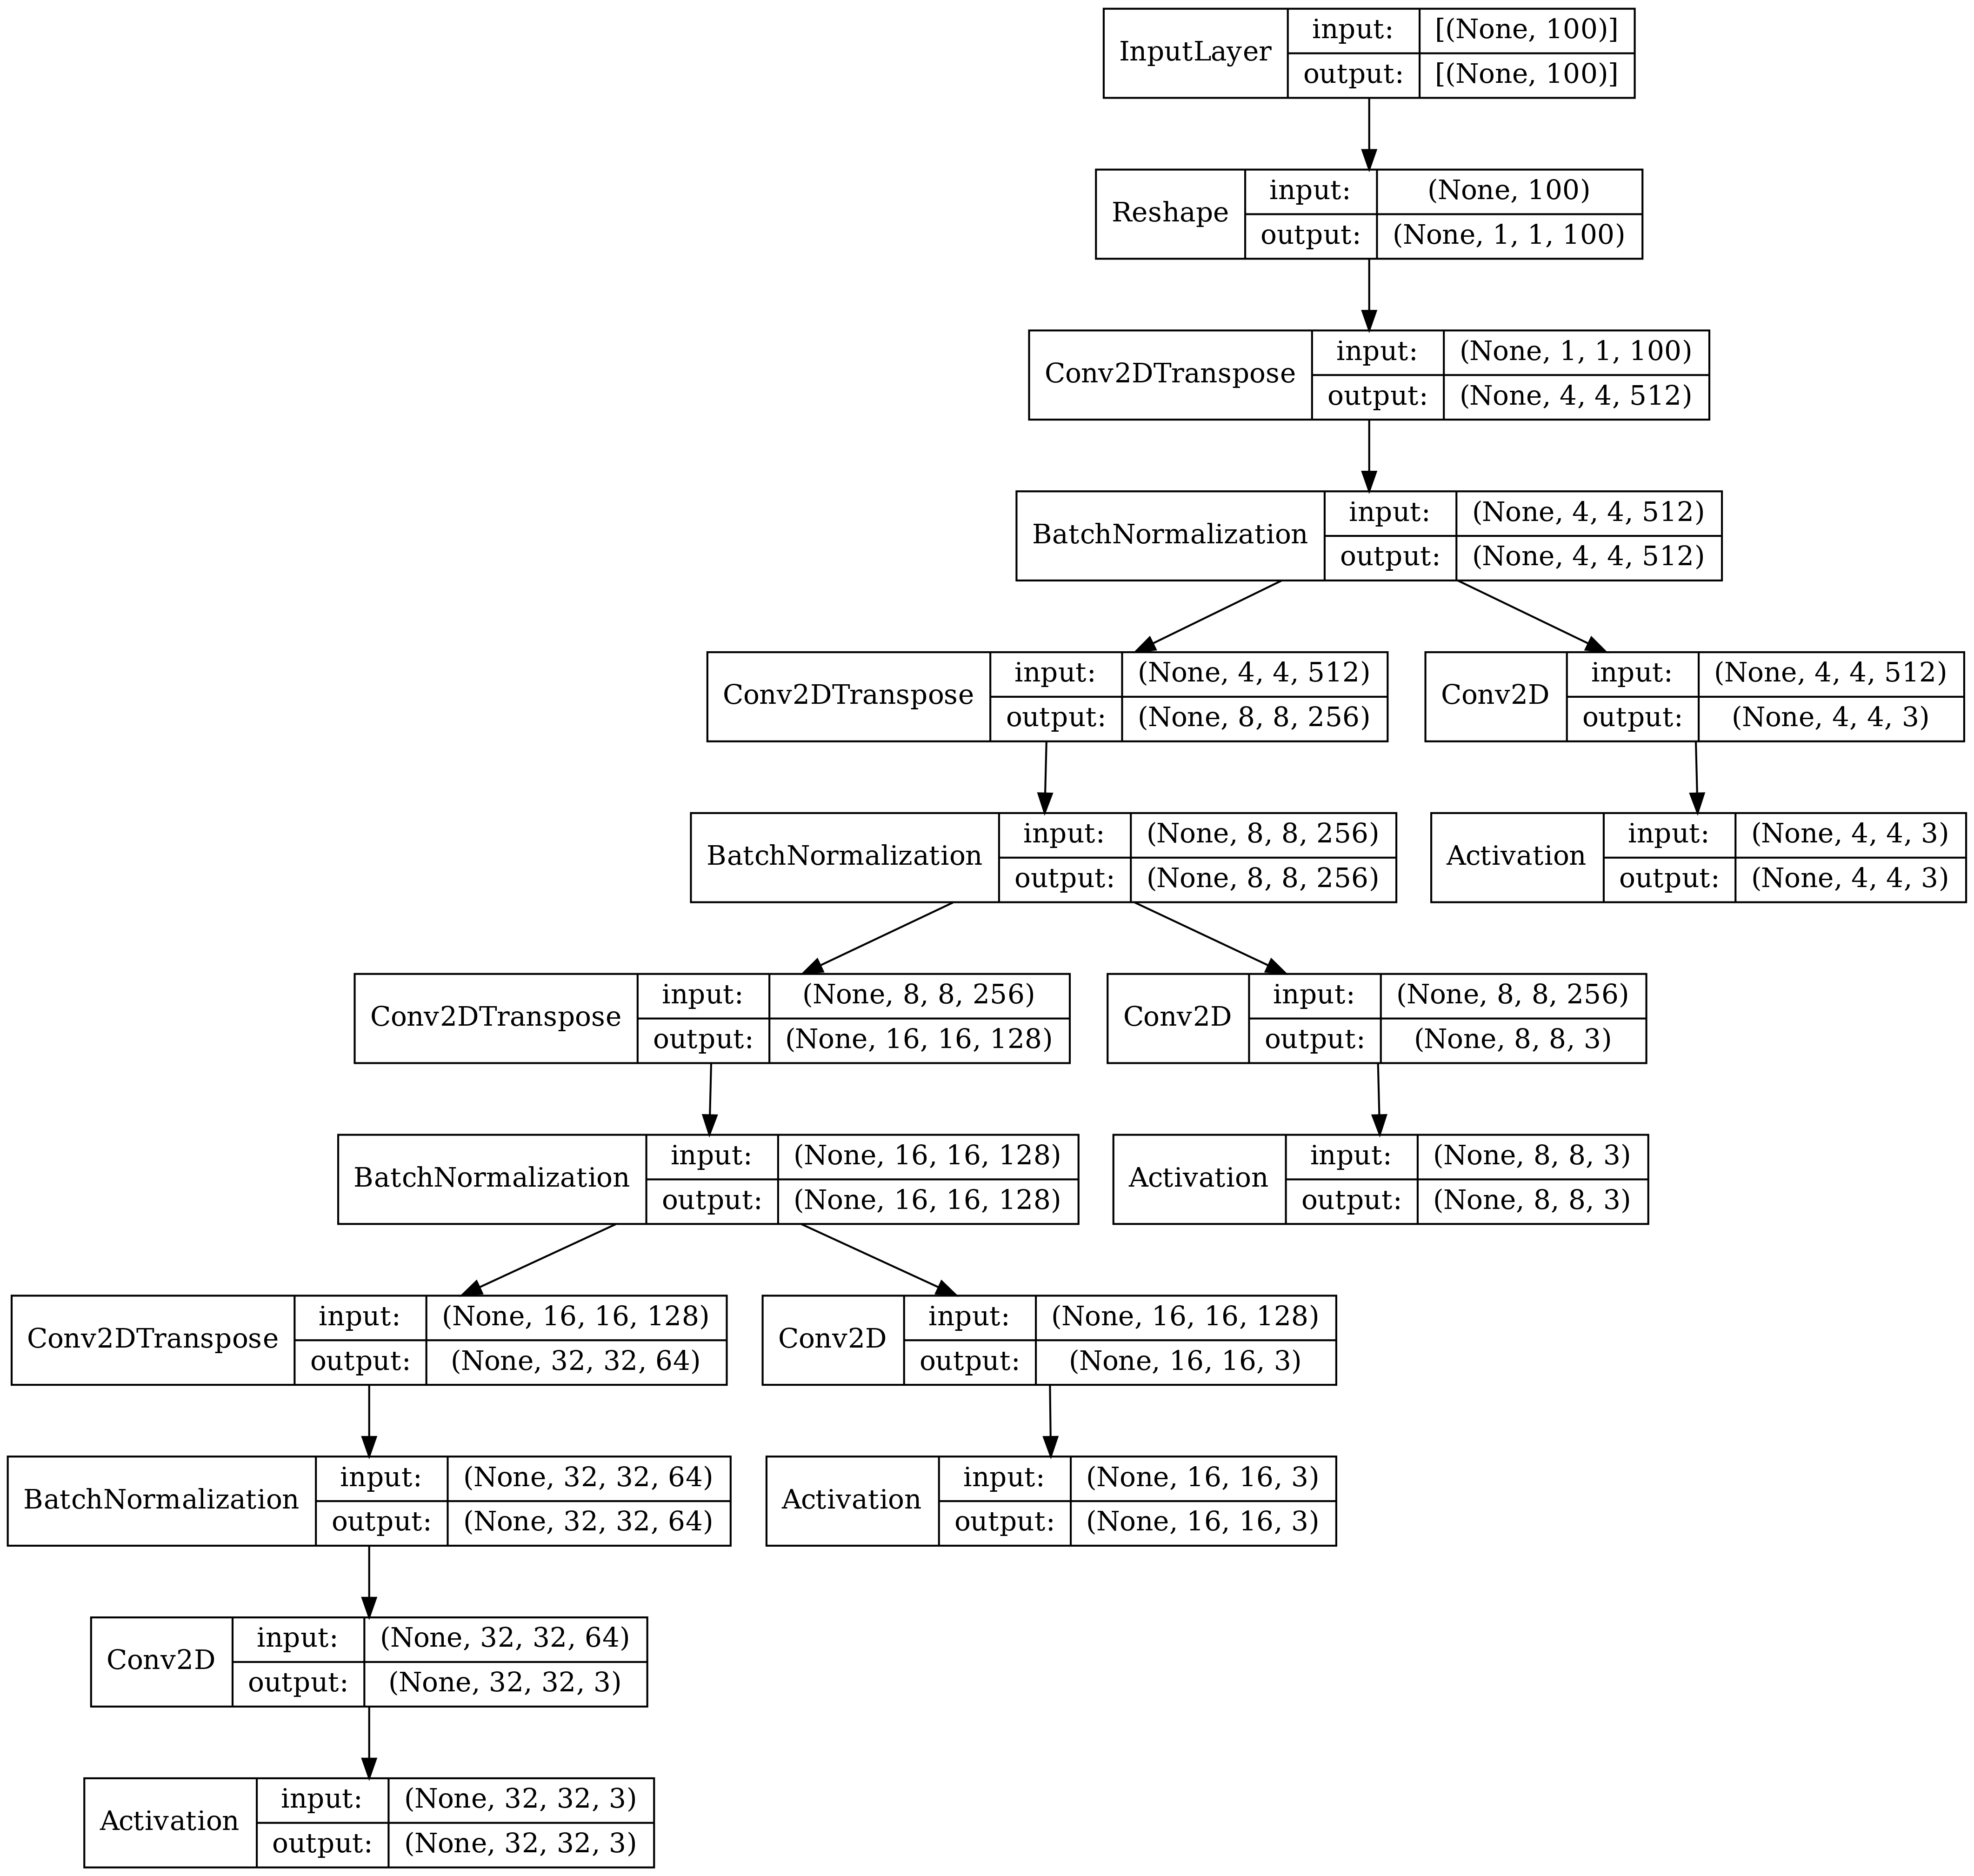
\includegraphics[width=15cm]{images/msgGenerator.png}
	\caption{Generátor több kimenettel, $32 \times 32$ maximális felbontással}
	\label{fig:msgGenerator}
\end{figure}

A Diszkriminátor modell architektúrája további módosításokat igényel. A bemeneteinek száma meg fog egyezni a Generátor kimeneteinek számával, a kapott képeket pedig a megfelelő helyre, a belső reprezentációihoz fűzi hozzá. A bemenetekből \textit{fromRGB} réteggel nyeri ki a feature-öket az összefűzéshez. Ezen konvolúciós rétegek feladata, hogy a három színcsatornával rendelkező képeket olyan reprezentációvá alakítsa át, amely az adott szint csatornaszámával megegyező csatornákat tartalmaz. Ezt úgy éri el, hogy a filterek számát a kívánt csatornaszámra állítjuk és "same" padding-et alkalmazunk $ 1 \times 1 $ stride értékek mellett. A kernelméret jelen esetben $ 3 \times 3 $-as, mivel ezen új rétegek a megnövekedett filterszámokkal igen sok további hiperparamétert adnak az eredeti modellhez.
Az egyértelműség érdekében a \textit{fromRGB} rétegek paraméterei a következő táblázatban is összefoglalásra került:

\small{
	\begin{center}
		\begin{tabular}{@{\extracolsep{6pt}} c c c c c }
			\hline
			\multicolumn{5}{l}{\textbf{\textit{fromRGB} konvolúciós réteg}} \\
			\hline
			Filterek száma & Kernelméret & Strides & Padding & Aktivációs függvény\\
			\cline{1-1} \cline{2-2} \cline{3-3} \cline{4-4} \cline{5-5}
			Az adott szinttel megegyező & $3 \times 3$ & $1 \times 1$ & "same" & nincsen\\
			\hline
		\end{tabular}
	\end{center}
}

\begin{figure}[h]
	\centering
	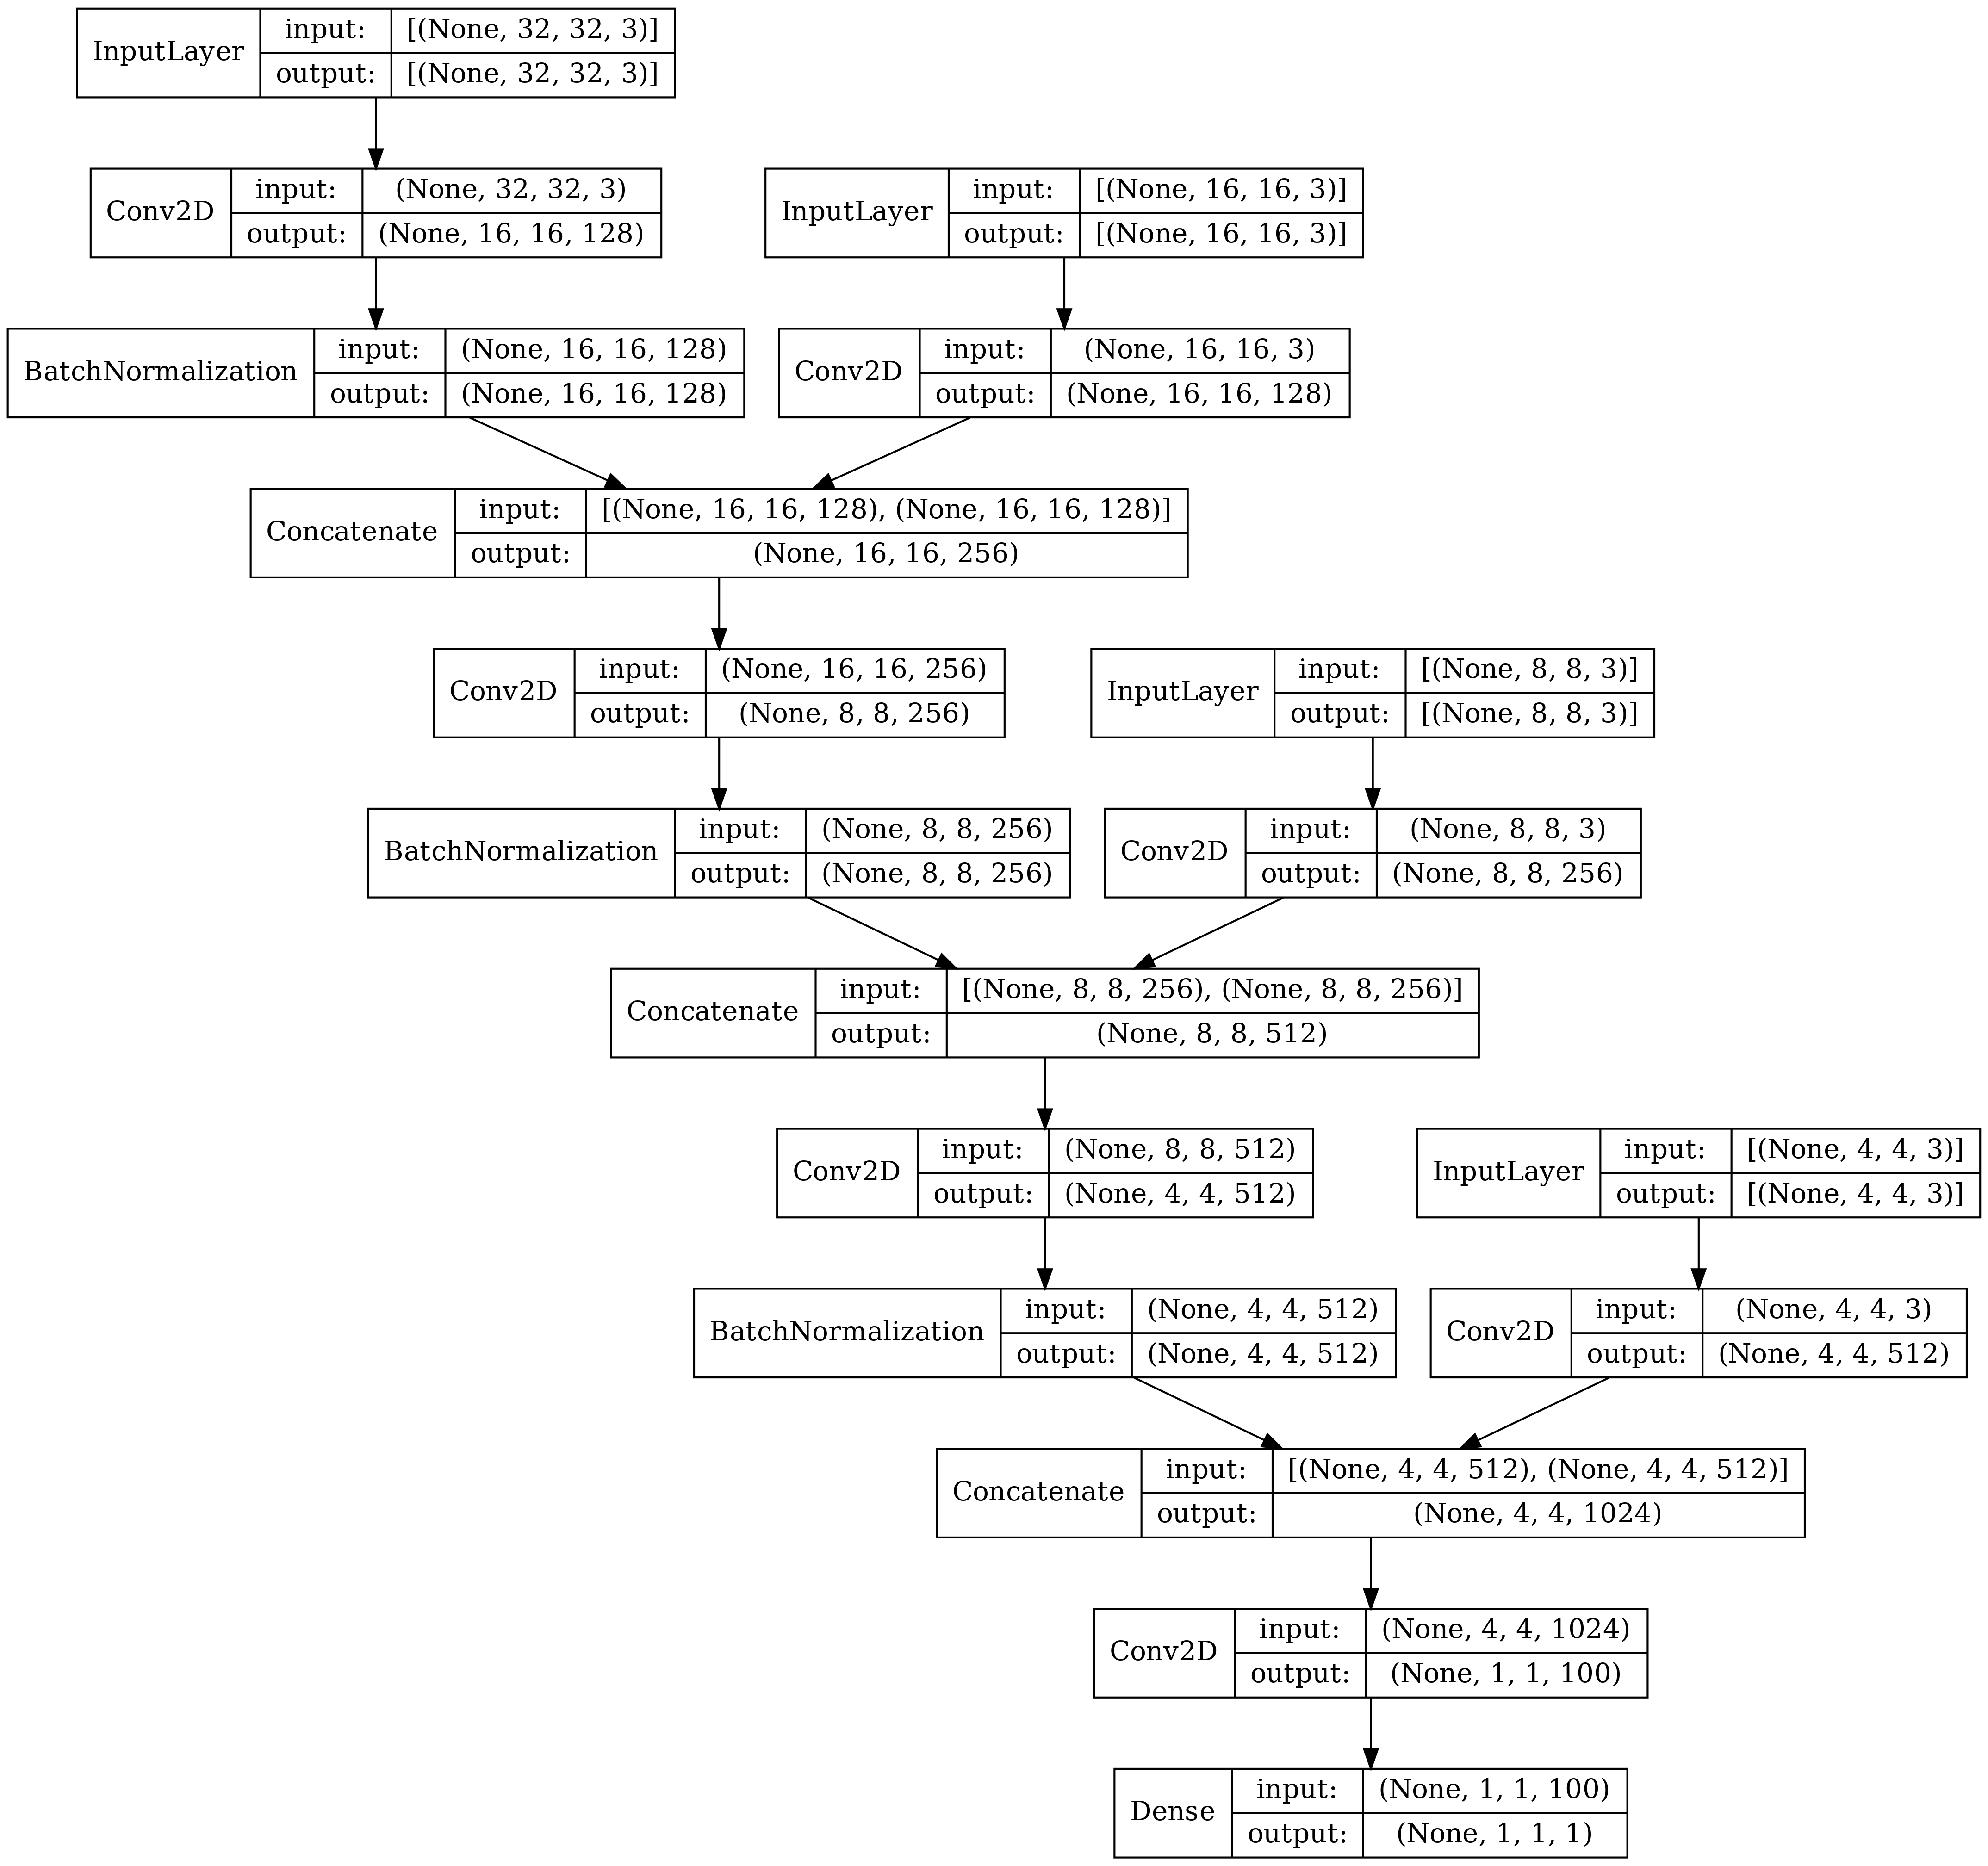
\includegraphics[width=15cm]{images/msgDiscriminator.png}
	\caption{Diszkriminátor több kimenettel $32 \times 32$ maximális felbontással}
	\label{fig:msgDiscriminator}
\end{figure}

A Diszkriminátor is megőrizte az eredeti felépítését (\ref{fig:msgDiscriminator}. ábra), viszont a \textit{fromRGB} rétegek igen sok további hiper-paramétert adnak hozzá a modellhez. Itt már milliós nagyságrendű új paraméter kerül a modellbe, és ezen kiegészítés hatására az eredetileg 3,5 millió paraméterrel rendelkező modell máris 7,1 millió paraméterrel rendelkezik. Így nem érvényesül a korábban felállított tükörkép-szerkezet, vagyis amikor a Diszkriminátor a Generátor fordítottja. A \textit{fromRGB} rétegek filtereinek számának hatására nő meg a paraméterek száma ilyen nagy mértékben. A módszert bemutató cikkben többféle módon is vizsgálták a bemenet összefűzés előtti feldolgozását. A nyers bemeneti képeken nem alkalmaztak végül transzformációt, és a cikkben felvázolt architektúrához az nyújtotta a legjobb megoldást. A saját implementációmat is ilyen módon készítettem el kezdetben. Viszont azt figyeltem meg, hogy csupán a nyers képek hozzáfűzése mellett a modell először a legnagyobb felbontású képeket tanulja meg megfelelően kigenerálni és a tanítás során igen lassan kerülnek a súlyok olyan állapotban, hogy az alsóbb rétegek is megfelelően megtanulják a kimenet elkészítését. A legkisebb felbontású kimeneten látszólag nem is tanult a modell, csupán random zaj jelent meg. Az architektúrámra alkalmazva a \textit{fromRGB} rétegeket megoldotta a legalsó rétegek tanulási problémáját.

\begin{figure}[h]
	\centering
	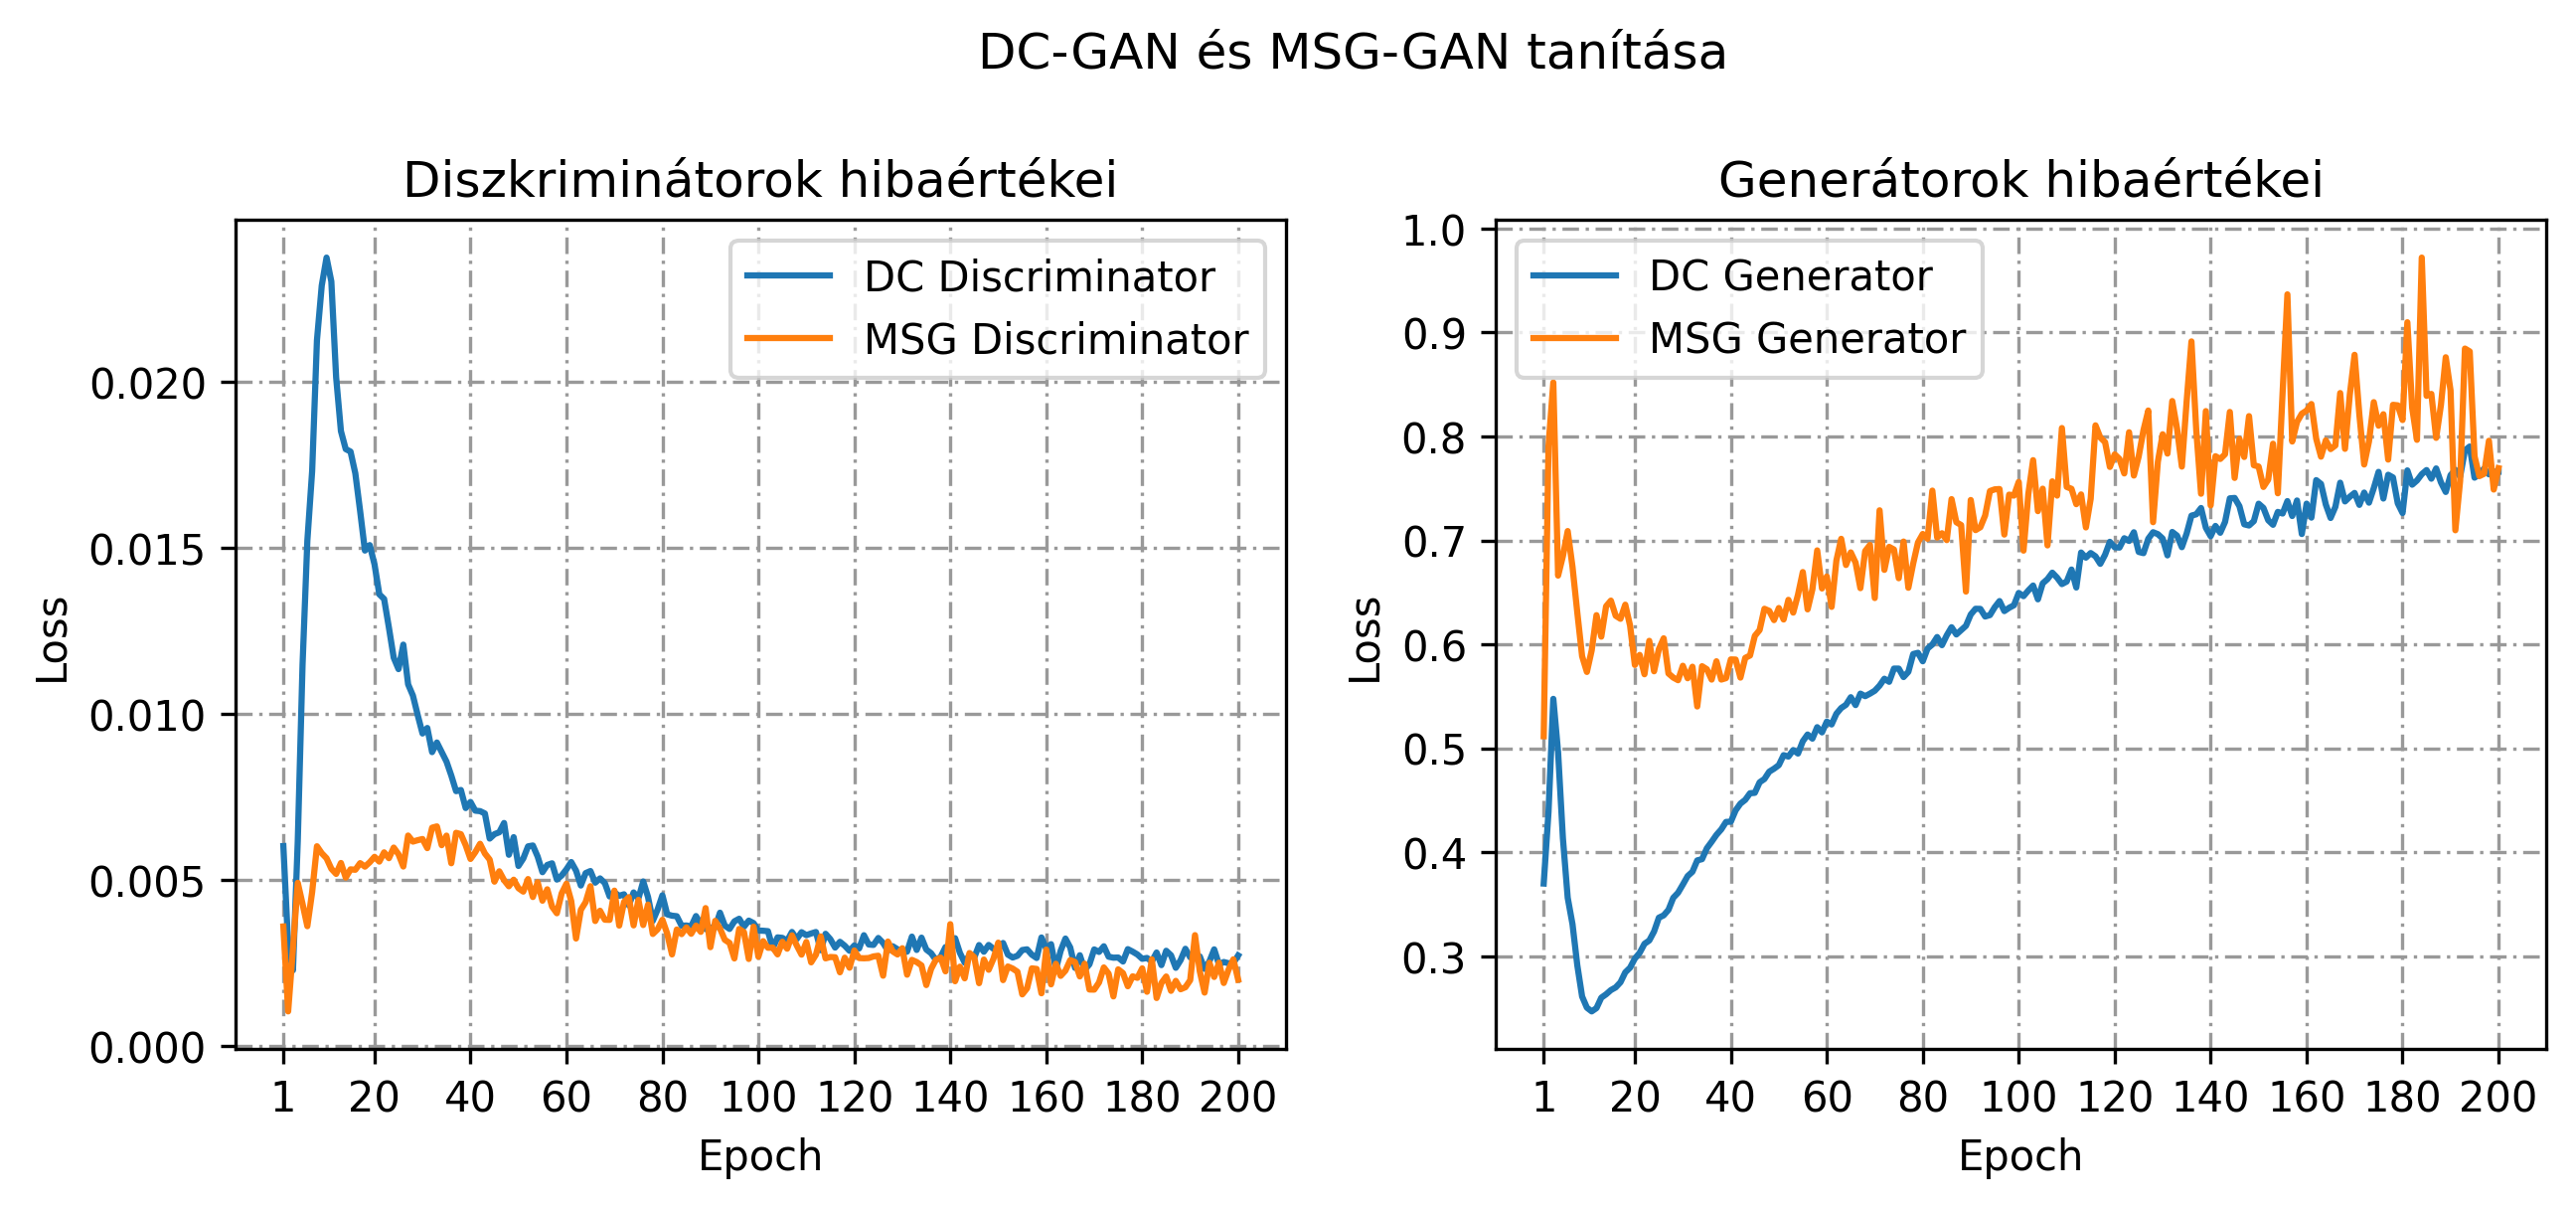
\includegraphics[width=15cm]{images/dc_vs_msg.png}
	\caption{A mély konvolúciós GAN és az MSG GAN tanítása során mért hibaértékek az AFHQ adathalmazon tanítva}
	\label{fig:dcvsmsg}
\end{figure}

\Aref{fig:dcvsmsg}. ábrán megfigyelhetők az eredeti és a kibővített modell Generátorainak és Diszkriminátorainak hibafüggvényei. Narancssárga színnel figyelhetjük meg az újonnan bemutatott modell hibaértékeit a tanulás alatt. A tanítás előrehaladtával hajlamosabb az oszcillációra a modell, viszont ami az ábrán még megfigyelhető, hogy a hibák értéktartománya sokkal szűkebb a Diszkriminátor és a Generátor esetében is.

\begin{figure}[h]
	\centering
	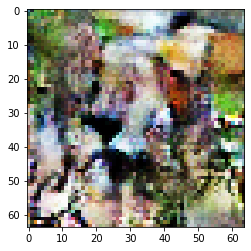
\includegraphics[width=5cm]{images/collapsed_mode.png}
	\caption{Egy "összeomlott-mode" a generátorban}
	\label{fig:collapsed_mode}
\end{figure}

Ezen kibővítés sem tökéletes. Az egyik, AFHQ adathalmazon betanított modell esetében a képek generálása során felfigyeltem egy visszatérő képre, amelyen érdekes mintázatok jelentek meg, viszont nem hasonlít az adathalmaz egyik elemére sem. A jelenségre, a mode-collapse fejezetben is említett, \textit{lokális mode} vagy \textit{összeomlott-mode}-ként is hivatkozhatunk. A látens tér bizonyos tartományában mintavételezett pontokra ugyanazt a képet generálja ki a modell, viszont a további pontokat nézve nem figyelhető meg semmiféle ismétlődő mintázat vagy egyéb mode-collapse-re utaló anomália. \Aref{fig:collapsed_mode}. ábrán látható egy példa az összeomlott-mode-ra. 

\Aref{fig:msg_output}. ábrán a Generátor kimeneteit figyelhetjük meg $4 \times 4$-es felbontástól egészen a $64 \times 64$ felbontásokig. Ezen ábrára tekintve érthető meg igazán a technika mögötti gondolat: a globális összefüggőségek az alacsonyabb felbontások mellett betanult jellegzetességek hatására alakul ki. A magasabb felbontásokon pedig az egyes képrészek részletességeinek növelése történik.

\begin{figure}[h]
	\centering
	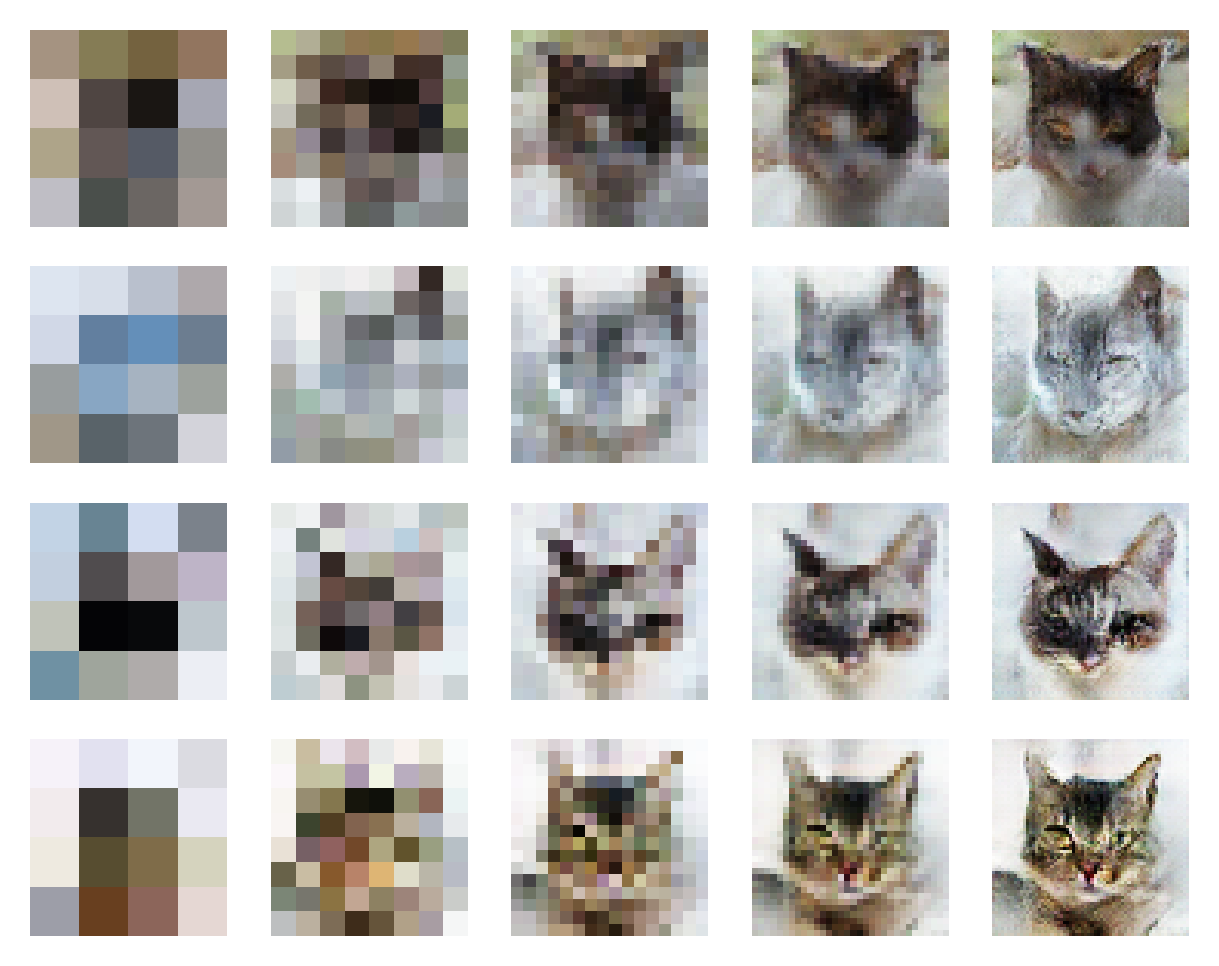
\includegraphics[width=12cm]{images/msg_output.png}
	\caption{Példa a Generátor kimeneteire $64 \times 64$ maximális felbontás mellett}
	\label{fig:msg_output}
\end{figure}

Az eredeti és ezen új modell teljesítményének méréséhez az Inception Score és a Fréchet Inception Distance metrikákat alkalmaztam. A méréshez a Cifar10 és az AFHQ adathalmaz elemein tanult mély konvolúciós (DC-GAN) és Multi Scale Gradient (MSG-GAN) generátorait használtam fel. A méréshez egységesen 10000 mintát generáltam mind a négy modellhez a tanításhoz is használt normális eloszlásból kapott látens vektorokkal. A mérés eredménye az alábbi táblázatban figyelhető meg.

\begin{center}
	\begin{tabular}{@{\extracolsep{6pt}} l c c c c }
		\hline
		& \multicolumn{2}{c}{\textbf{IS}} & \multicolumn{2}{c}{\textbf{FID}}\\
		\cline{2-3} \cline{4-5}
		& Cifar10 & AFHQ & Cifar10 & AFHQ\\
		\hline
		DC-GAN & $5.4394 \pm 0.276$ & $4.9611 \pm 0.1464$ & $51.4926$ & $635.8320$\\
		MSG-GAN & $5.9588 \pm 0.1273$ & $6.0283 \pm 0.2169$ & $43.5502$ & $596.7116$\\
		\hline
	\end{tabular}
\end{center}

\noindent Az IS esetében a magasabb érték jelent jobb eredményt, az FID-nál pedig az alacsonyabb eredmény jelent jobb teljesítményt. A mérés alapján az alkalmazott kiegészítés a modell előnyére vált, viszont nagymértékű javulás nem tapasztalható.
